% ------------------------------------------------
%
%論文內容次序:
% 1.考試合格證明
% 2.中英文摘要(論文以中文撰寫者須附英文延伸摘要)
% 3.誌謝
% 4.目錄
% 5.表目錄
% 6.圖目錄
% 7.符號
% 8.主文
% 9.參考文獻
% 10.附錄
%
% 註: 參考文獻書寫注意事項:
% (1).
%    文學院之中文文獻依分類及年代順序排列。
%    其他學院所之文獻依英文姓氏第一個字母
%    (或中文姓氏第一個字筆劃)及年代順序排列。
%
% (2).
%    期刊文獻之書寫依序為:
%        姓名、文章名稱、期刊名、卷別、期別、頁別、年代。
%
% (3).
%    書寫之文獻依序為:
%        姓名、書名、出版商名、出版地、頁別、年代。
%
% ------------------------------------------------

% 封面內頁 Inner Cover
%
% 封面: 顯示所有封面內容, 沒有學校Logo
%     主要用在印刷版, 如精裝版 或 平裝版
%     (使用cover.tex來產生)
%
% 內頁: 顯示所有封面內容, 沒有學校Logo
%     主要用在電子版 + 印刷版
%
% 只要是印刷版, 不論是精裝版或平裝版, 都是 封面 (殼/皮) + 內頁.
% 只有在電子版時, 第一頁就是封面內頁.

\DisplayInnerCover

% ------------------------------------------------

% 學位考試論文證明書
\DisplayOral

% ------------------------------------------------

% 摘要 Abstract
% 除了外籍生, 本地生和僑生都是要編寫中文和英文摘要
% 論文以中文撰寫須以英文補寫 800 至 1200 字數的英文延伸摘要 (Extended Abstract)
% 詳細可看附件的學校要求或看example中的英文延伸摘要

%% ------------------------------------------------
\StartAbstractChi
% ------------------------------------------------

除了外籍生, 本地生和僑生都是要編寫中文和英文摘要. 論文以中文撰寫須以英文補寫 800 至 1200 字數的英文延伸摘要 (Extended Abstract), 如需要的話請修改`./context/abstract/extended.tex'.

外籍生則可免填中文摘要, 而在上傳時網頁資訊需填上`NONE'.\\

% ------------------------------------------------
\EndAbstractChi
% ------------------------------------------------
             % 中文版
% ------------------------------------------------
\StartAbstract
% ------------------------------------------------

Fake news has become a critical threat to information integrity and social stability, particularly in few-shot scenarios where limited labeled data is available for emerging topics or misinformation campaigns. Traditional fake news detection methods rely heavily on user propagation patterns or require extensive labeled datasets, making them impractical for real-world deployment where such data is scarce or unavailable. This thesis presents GemGNN (Generative Multi-view Interaction Graph Neural Networks), a novel framework for few-shot fake news detection that addresses these fundamental limitations through content-based graph neural network modeling.

Our approach introduces three key innovations: First, we develop a generative user interaction simulation method using Large Language Models (LLMs) to synthesize diverse user interactions with multiple tones (neutral, affirmative, skeptical), effectively overcoming the dependency on real user propagation data. Second, we propose a Test-Isolated K-Nearest Neighbor (KNN) edge construction strategy that prevents information leakage between test nodes, ensuring more realistic and robust evaluation in few-shot scenarios. Third, we implement a multi-view graph construction approach that splits news embeddings into multiple semantic perspectives, combined with multi-graph training for enhanced data augmentation.

The GemGNN framework employs Heterogeneous Graph Attention Networks (HAN) to model complex relationships between news articles and generated user interactions through dynamic attention mechanisms. Our transductive learning approach leverages both labeled and unlabeled data during message passing while restricting loss computation to labeled nodes only, maximizing the utility of limited supervision.

Extensive experiments on the FakeNewsNet datasets (PolitiFact and GossipCop) demonstrate that GemGNN significantly outperforms state-of-the-art methods across various few-shot configurations (K=3-16). Our method achieves superior F1-scores compared to traditional approaches (MLP, LSTM), transformer-based models (BERT, RoBERTa), large language models (LLaMA, Gemma), and existing graph-based methods (Less4FD, HeteroSGT). Comprehensive ablation studies validate the effectiveness of each component, showing that the combination of generative interactions, test-isolated KNN, and multi-view construction provides substantial improvements in few-shot fake news detection performance.

The contributions of this work establish a new paradigm for content-based fake news detection that eliminates dependency on user behavior data while maintaining superior performance in data-scarce scenarios, making it particularly suitable for privacy-sensitive applications and emerging misinformation detection tasks.

% ------------------------------------------------
\EndAbstract
% ------------------------------------------------
             % 英文版
%% ------------------------------------------------
\StartExtendedAbstract
% ------------------------------------------------

\ExtAbstractSummary{%
The summary is a short, informative abstract of no more than 250 words. References should not be cited. The summary should (1) state the scope and objectives of the research, (2) describe the methods used, (3) summarize the results, and (4) state the principal conclusions. Text of the summary should be 12 pt Times New Roman font, single-spaced and justified. A single line space should be left below the title `SUMMARY'. Leave a single line space above the key words listed below.
} % End of \ExtAbstractSummary{}

% ------------------------------------------------

\ExtAbstractChapter{INTRODUCTION}
The purpose of the introduction is to tell readers why they should want to read your thesis/ dissertation. This section should provide sufficient background information to allow readers to understand and evaluate the paper's results.

The introduction should (1) present the nature and scope of the problem, (2) review related literature, (3) describe the materials used and method(s) of the study, and (4) describe the main results of the study.

All text in the main body of the extended abstract should be 12 pt Times New Roman font, single-spaced and justified. Main headings are placed in the centre of the column, in capital letters using 12 pt Times New Roman Bold font. Subheadings are placed on the left margin of the column and are typed in 12 pt Times New Roman Bold font.

% ------------------------------------------------

\ExtAbstractChapter{MATERIALS AND METHODS}
There is flexibility as to the naming of the section (or sections) that provide information on the method(s) or theories employed. The methodology employed inthe work must be described in sufficient detail or with sufficient references so that the results could be duplicated.

Your materials should be organised carefully. Include all the data necessary to support your conclusions, but exclude redundant or unnecessary data.

% ------------------------------------------------

\ExtAbstractChapter{RESULTS AND DISCUSSION}
The results and discussion sections present your research findings and your analysis of those findings. The results of experiments can be presented as tables or figures.

% ------------------------------------------------

\ExtAbstractSection{Figures and Tables}
Figures may be integrated within the results section of the extended abstract, or they can be appended to the end of the written text. Figures should be black \& white. They should be no wider than the width of the A4 page.

Tables can be created within Word. As noted for figures above, if a table is to be placed within the text, it can be no wider than the width of the A4 page. Larger tables will need to be placed at the end of the abstract.

Figures and tables should be numbered according to the order they are referenced in the paper. Figures and tables should be referred to by their number in the text. When referring to figures and tables in the text, spell out and capitalize the word Figure or Table. All figures and tables must have captions.

% ------------------------------------------------

\ExtAbstractSection{Captions}
Captions should clearly explain the significance of the figure or table without reference to the text. Details in captions should not be restated in the text. Parameters in figure captions should be included and presented in words rather than symbols.

Captions should be placed directly above the relevant table and beneath the relevant figure. The caption should be typed in 12 pt Times New Roman Bold font. Spell out the word `Table' or `Figure' in full. An example table and a figure follow.

% ------------------------------------------------

\InsertTable
  [caption={Specifications of the engine}]
  {
    \begin{tabular}{llll}
    \hline
    Engine &  &  & OPEL Astra C16SE \\ \hline
    Displacement (cc) &  &  & 1598 \\
    Bore x stroke(mm x mm) &  &  & 79 x 81.5 \\
    Value mechanism &  &  & SOHC \\
    Number of valves &  &  & Intake 4, exhaust 4 \\
    Compression ratio &  &  & 9.8:1 \\
    Torque &  &  & 135/3400 Nm/rpm \\
    Power &  &  & 74/5800 kW/rpm \\
    Ignition sequence &  &  & 1-3-4-2 \\
    Spark plug &  &  & BPR6ES \\
    Fuel &  &  & 95 unleaded gasoline \\
    Cylinder arrangment &  &  & In-line 4 cylinders \\ \hline
    \end{tabular}
  } % End of  \InsertTable{}

\InsertFigure
  [scale=0.5,
    caption={HC emission as a function of equivalence ratio}]
  {./example/abstract/pic/extended-abstract-2.jpg}

% ------------------------------------------------

\ExtAbstractChapter{CONCLUSION}
This section should include (1) the main points of your paper and why they are significant, (2) any exceptions to, problems with, or limitations to your argument, (3) agreements or disagreements with previously published work, (4) theoretical and practical implications of the work, and (5) conclusions drawn.

% ------------------------------------------------
\EndExtendedAbstract
% ------------------------------------------------
        % 英文延伸摘要

% ------------------------------------------------

% 誌謝 Acknowledgments
% 誌謝正常應該只要寫一種版本就可,
% 提供2種以自行選擇所顯示的語言.
% 2種同時編寫都是可以的.

%% ------------------------------------------------
\StartAcknowledgmentsChi
% ------------------------------------------------

在這邊寫你的感謝 (對父母, 老師, 同學, 朋友等的感謝).

% ------------------------------------------------
\EndAcknowledgments
% ------------------------------------------------
             % 中文版
% ------------------------------------------------
\StartAcknowledgments
% ------------------------------------------------

Thanks someone you want in here.

% ------------------------------------------------
\EndAcknowledgments
% ------------------------------------------------
             % 英文版

% ------------------------------------------------

% 目錄 (內容, 圖表和圖片) Index of contents, tables and figures.
% 內容會自動產生 The indices will generate in automate.
\DisplayIndex                 % 顯示索引
\DisplayTablesIndex   % 顯示表格索引
\DisplayFiguresIndex  % 顯示圖片索引

% ------------------------------------------------

% Nomenclature
\StartNomChapter{Nomenclature}{chapter:nomenclature}

%%https://www.artofproblemsolving.com/wiki/index.php/LaTeX:Symbols
%https://www.sharelatex.com/learn/List_of_Greek_letters_and_math_symbols
%https://oeis.org/wiki/List_of_LaTeX_mathematical_symbols
% ------------------------------------------------

\InsertTable
  {
    \begin{tabular}{C{0.2\textwidth} L{0.4\textwidth}}
    \hline
    \underline{Symbol} & \centerline{\underline{Description}}\\
        $\alpha$ & Symbol of alpha \\
        $\beta$ & \\
        $\gamma$ & Gamma\\
    \hline
    \end{tabular}
  }

\EmptyLine

\InsertTable
  [pos=bottom, nomtitle={List of common physics notations}]
  {
    \begin{tabular}{C{0.2\textwidth} C{0.4\textwidth} C{0.35\textwidth}}
    \hline
    \underline{Symbol} & \underline{Meaning} & \underline{SI unit of measure} \\
        $g$ & Standard gravity & $9.80665 m/s^2$ \\
        $c$ & Speed of light & $\approx3.00\times108 m/s$  \\
        $l$ & Length & meter (m) \\
 	  \hline
    \end{tabular}
  }

% ------------------------------------------------

\EndNomChapter


% ------------------------------------------------

% Chapter 1: Introduction
% ------------------------------------------------
\StartChapter{Introduction}{chapter:introduction}
% ------------------------------------------------

\section{Research Background and Motivation}

In the digital age, the proliferation of fake news has emerged as one of the most pressing challenges threatening information integrity and democratic discourse. According to Vosoughi et al. \cite{vosoughi2018spread}, false news spreads six times faster than true news on social media platforms, reaching more people and penetrating deeper into social networks. This phenomenon has far-reaching consequences, from influencing electoral outcomes to undermining public health responses during critical events such as the COVID-19 pandemic.

Traditional approaches to fake news detection have relied heavily on two primary paradigms: content-based analysis and propagation-based modeling. Content-based methods analyze linguistic features, semantic patterns, and textual inconsistencies within news articles, while propagation-based approaches examine how information spreads through social networks by modeling user interactions, sharing patterns, and network topology. However, both paradigms face significant limitations in real-world deployment scenarios.

The most critical challenge in contemporary fake news detection is the few-shot learning problem, where detection systems must accurately classify news articles with minimal labeled training data. This scenario is particularly common when dealing with emerging topics, breaking news events, or novel misinformation campaigns where extensive labeled datasets are not readily available. Traditional deep learning approaches, which typically require thousands of labeled examples per class, fail to perform adequately in such data-scarce environments.

Furthermore, existing propagation-based methods, while often achieving high performance, suffer from fundamental practical limitations. These approaches require access to comprehensive user interaction data, including social network structures, user profiles, and temporal propagation patterns. Such data is increasingly difficult to obtain due to privacy regulations, platform restrictions, and the real-time nature of misinformation spread. Additionally, these methods are vulnerable to sophisticated adversarial attacks where malicious actors can manipulate propagation patterns to evade detection.

\section{Problem Statement and Challenges}

This thesis addresses the fundamental problem of few-shot fake news detection in scenarios where traditional propagation data is unavailable or unreliable. Formally, we define our problem as follows:

\textbf{Problem Definition:} Given a small set of labeled news articles $\mathcal{L} = \{(x_i, y_i)\}_{i=1}^{K \times C}$ where $K$ represents the number of examples per class and $C$ denotes the number of classes (real/fake), and a larger set of unlabeled news articles $\mathcal{U} = \{x_j\}_{j=1}^{M}$, the objective is to learn a classifier $f: \mathcal{X} \rightarrow \mathcal{Y}$ that can accurately predict labels for test instances $\mathcal{T} = \{x_k\}_{k=1}^{N}$ where $K \ll M$ and $K \ll N$.

The core challenges that motivate this research include:

\textbf{Limited Labeled Data:} Few-shot scenarios typically provide only 3-16 labeled examples per class, insufficient for training robust deep learning models using conventional approaches. This data scarcity leads to overfitting, poor generalization, and unstable performance across different domains.

\textbf{Absence of Propagation Information:} Real-world deployment often lacks access to user interaction data due to privacy constraints, platform limitations, or the time-sensitive nature of misinformation detection. Existing propagation-based methods become inapplicable in such contexts.

\textbf{Semantic Complexity:} Fake news articles often exhibit sophisticated linguistic patterns and may contain accurate factual information presented in misleading contexts. Simple content-based features fail to capture these nuanced semantic relationships.

\textbf{Domain Generalization:} Models trained on specific topics or domains often fail to generalize to emerging misinformation patterns or novel subject areas, limiting their practical applicability.

\textbf{Evaluation Realism:} Many existing few-shot learning approaches suffer from information leakage between training and test sets, leading to overly optimistic performance estimates that do not reflect real-world deployment scenarios.

\section{Research Contributions}

This thesis presents GemGNN (Generative Multi-view Interaction Graph Neural Networks), a novel framework that addresses the aforementioned challenges through several key contributions:

\textbf{Generative User Interaction Simulation:} We introduce the first approach to synthesize realistic user interactions using Large Language Models (LLMs), specifically leveraging Gemini to generate diverse user responses with multiple emotional tones (neutral, affirmative, skeptical). This innovation eliminates the dependency on real propagation data while maintaining the benefits of interaction-based modeling.

\textbf{Test-Isolated KNN Edge Construction:} We develop a novel graph construction strategy that prevents information leakage between test nodes through strict isolation constraints. This approach ensures more realistic evaluation by prohibiting test nodes from connecting to each other, addressing a critical flaw in existing graph-based few-shot learning methods.

\textbf{Multi-View Graph Architecture:} We propose a multi-view learning framework that partitions news embeddings into multiple semantic perspectives, enabling the model to capture diverse aspects of news content. Each view constructs its own graph structure, and multiple graphs are trained simultaneously to provide comprehensive data augmentation.

\textbf{Enhanced Heterogeneous Graph Neural Networks:} We design a specialized HAN-based architecture that effectively models the complex relationships between news articles and generated user interactions through type-specific attention mechanisms and hierarchical aggregation strategies.

\textbf{Comprehensive Evaluation Framework:} We establish rigorous experimental protocols that ensure fair comparison with existing methods while maintaining realistic few-shot learning constraints across multiple datasets and evaluation metrics.

\section{Thesis Organization}

The remainder of this thesis is organized as follows:

\textbf{Chapter 2: Related Work} provides a comprehensive review of existing fake news detection methods, including traditional feature-engineering approaches, deep learning techniques, graph-based methods, and few-shot learning strategies. We analyze the limitations of current approaches and position our work within the broader research landscape.

\textbf{Chapter 3: Background and Preliminaries} introduces the fundamental concepts underlying our approach, including few-shot learning formulations, graph neural network architectures, and problem notation. This chapter establishes the theoretical foundation necessary for understanding our methodology.

\textbf{Chapter 4: Methodology} presents the complete GemGNN framework, detailing the generative user interaction simulation, test-isolated KNN construction, multi-view graph architecture, and the heterogeneous graph neural network design. We provide comprehensive algorithmic descriptions and theoretical justifications for each component.

\textbf{Chapter 5: Experimental Setup} describes our experimental methodology, including dataset preprocessing, baseline method implementations, evaluation protocols, and hyperparameter configurations. We ensure reproducibility and fair comparison across all experimental conditions.

\textbf{Chapter 6: Results and Analysis} presents comprehensive experimental results, including main performance comparisons, ablation studies, and detailed analysis of model behavior. We provide insights into why our approach succeeds in few-shot scenarios and identify the key factors contributing to performance improvements.

\textbf{Chapter 7: Conclusion and Future Work} summarizes our contributions, discusses the implications of our findings, acknowledges current limitations, and outlines promising directions for future research in few-shot fake news detection.

% ------------------------------------------------
\EndChapter
% ------------------------------------------------


% Chapter 2: Related Work  
% ------------------------------------------------
\StartChapter{Related Work}{chapter:related-work}
% ------------------------------------------------

Write your relatd work here.

% ------------------------------------------------
\EndChapter
% ------------------------------------------------


% Chapter 3: Background and Preliminaries
% ------------------------------------------------
\StartChapter{Background and Preliminaries}{chapter:background}
% ------------------------------------------------

This chapter provides the theoretical foundation necessary for understanding our GemGNN framework. We introduce fundamental concepts in few-shot learning, graph neural networks for text classification, and establish the formal problem formulation with mathematical notation used throughout this thesis.

\section{Few-Shot Learning Fundamentals}

Few-shot learning represents a paradigm shift from traditional machine learning approaches that require extensive labeled datasets. In few-shot scenarios, models must achieve strong performance with minimal supervision, making them particularly relevant for real-world applications where labeling is expensive or impractical.

\subsection{Problem Formulation}

\textbf{Formal Definition:} Few-shot learning is a machine learning framework where an AI model learns to make accurate predictions by training on a very small number of labeled examples per class. Formally, given a support set $\mathcal{S} = \{(x_i, y_i)\}_{i=1}^{K \times N}$ containing $K$ labeled examples for each of $N$ classes, the objective is to learn a classifier $f: \mathcal{X} \rightarrow \mathcal{Y}$ that can accurately predict labels for a query set $\mathcal{Q} = \{x_j\}_{j=1}^{M}$.

\textbf{N-way K-shot Classification:} The standard formulation for few-shot learning is N-way K-shot classification, where $N$ represents the number of classes and $K$ denotes the number of labeled examples per class. In our fake news detection task, we focus on 2-way K-shot learning with $K \in \{3, 4, 8, 16\}$, where the two classes represent real and fake news respectively.

\textbf{Support and Query Sets:} The support set $\mathcal{S}$ contains the limited labeled examples available for training, while the query set $\mathcal{Q}$ contains unlabeled instances that must be classified. In traditional few-shot learning, these sets are disjoint, but our transductive approach allows overlap between support and query sets during training while maintaining separation during evaluation.

\subsection{Challenges in Few-Shot Learning}

Few-shot learning presents several fundamental challenges that differentiate it from conventional machine learning:

\textbf{Limited Training Data:} Traditional deep learning requires thousands of labeled examples per class to achieve good performance. In few-shot scenarios with only 3-16 examples per class, models are highly prone to overfitting and struggle to learn generalizable patterns.

\textbf{High Variance:} The limited sample size leads to high variance in performance estimates. Small changes in the support set can dramatically affect model performance, making robust evaluation protocols crucial for reliable results.

\textbf{Class Imbalance:} Few-shot datasets often exhibit class imbalance, particularly in real-world scenarios where certain types of misinformation may be more prevalent than others. Standard loss functions may not be appropriate for such imbalanced settings.

\textbf{Domain Shift:} Models trained on few examples from specific domains often fail to generalize to new domains or emerging patterns not represented in the limited training data.

\textbf{Evaluation Challenges:} Proper evaluation of few-shot learning systems requires careful experimental design to avoid information leakage and ensure that performance estimates reflect real-world deployment scenarios.

\subsection{Few-Shot Learning Strategies}

Several general strategies have been developed to address few-shot learning challenges:

\textbf{Meta-Learning:} Meta-learning approaches, such as Model-Agnostic Meta-Learning (MAML), learn initialization parameters that can be quickly adapted to new tasks. The key insight is to learn how to learn rather than learning specific task solutions.

\textbf{Metric Learning:} These approaches learn embedding spaces where examples from the same class are close together and examples from different classes are far apart. Classification is performed by comparing query examples to support set prototypes.

\textbf{Data Augmentation:} Various augmentation strategies generate additional training examples from the limited support set through transformations, perturbations, or generative models.

\textbf{Transfer Learning:} Pre-trained models capture general knowledge that can be adapted to specific few-shot tasks through fine-tuning or feature extraction.

\textbf{Regularization:} Specialized regularization techniques prevent overfitting in few-shot scenarios by constraining model complexity or encouraging specific types of solutions.

\section{Graph Neural Networks for Text Classification}

Graph Neural Networks have emerged as a powerful paradigm for modeling structured data, with particular success in text classification tasks where relationships between documents provide valuable signal for classification.

\subsection{Message Passing Framework}

\textbf{Core Principle:} GNNs operate on the message passing framework where nodes iteratively update their representations by aggregating information from neighboring nodes. This process enables the model to capture both local neighborhood information and global graph structure through multiple iterations.

\textbf{General Formulation:} The message passing framework can be described through three key operations:

1. \textbf{Message Function:} $m_{ij}^{(l+1)} = M^{(l)}(h_i^{(l)}, h_j^{(l)}, e_{ij})$ computes messages between connected nodes, where $h_i^{(l)}$ represents the feature vector of node $i$ at layer $l$, and $e_{ij}$ represents edge features.

2. \textbf{Aggregation Function:} $a_i^{(l+1)} = A^{(l)}(\{m_{ij}^{(l+1)} : j \in \mathcal{N}(i)\})$ aggregates messages from all neighbors $\mathcal{N}(i)$ of node $i$.

3. \textbf{Update Function:} $h_i^{(l+1)} = U^{(l)}(h_i^{(l)}, a_i^{(l+1)})$ updates the node representation based on its current state and aggregated messages.

\textbf{Multi-Layer Architecture:} Multiple message passing layers enable nodes to receive information from increasingly distant neighbors, allowing the model to capture both local patterns and global graph structure.

\subsection{Graph Construction for Text}

\textbf{Document Graphs:} For text classification, documents are typically represented as nodes in a graph, with edges indicating various types of relationships such as semantic similarity, citation links, or co-occurrence patterns.

\textbf{Similarity-Based Construction:} The most common approach constructs edges between documents based on content similarity measures such as cosine similarity of embedding vectors. Documents with similarity above a threshold or among the top-k nearest neighbors are connected.

\textbf{Heterogeneous Graphs:} More sophisticated approaches construct heterogeneous graphs that include multiple node types (documents, words, authors, topics) and edge types (document-word, document-document, word-word), enabling richer modeling of text relationships.

\textbf{Dynamic Graph Construction:} Advanced methods adapt graph structure during training or inference, allowing the model to learn optimal connectivity patterns rather than relying on fixed similarity measures.

\subsection{Heterogeneous Graph Attention Networks}

HAN addresses the challenges of modeling heterogeneous graphs with multiple node and edge types through hierarchical attention mechanisms.

\textbf{Node-Level Attention:} For each edge type $\phi$, HAN computes attention weights between connected nodes:
\begin{equation}
\alpha_{ij}^{\phi} = \text{softmax}\left(\sigma\left(\mathbf{a}_{\phi}^T [\mathbf{W}_{\phi} \mathbf{h}_i \| \mathbf{W}_{\phi} \mathbf{h}_j]\right)\right)
\end{equation}

where $\mathbf{W}_{\phi}$ is the edge-type-specific transformation matrix, $\mathbf{a}_{\phi}$ is the attention vector, and $\|$ denotes concatenation.

\textbf{Semantic-Level Attention:} HAN aggregates information across different edge types using learned importance weights:
\begin{equation}
\beta_{\phi} = \frac{1}{|\mathcal{V}|} \sum_{i \in \mathcal{V}} \mathbf{q}^T \tanh(\mathbf{W} \cdot \mathbf{h}_i^{\phi} + \mathbf{b})
\end{equation}

where $\mathbf{h}_i^{\phi}$ represents the node embedding for edge type $\phi$.

\textbf{Final Representation:} The complete node representation combines information from all edge types:
\begin{equation}
\mathbf{h}_i = \sum_{\phi \in \Phi} \beta_{\phi} \mathbf{h}_i^{\phi}
\end{equation}

This hierarchical attention mechanism enables the model to learn both which neighbors are important for each edge type and which edge types are most relevant for the classification task.

\section{Problem Formulation and Notation}

We now formally define the few-shot fake news detection problem addressed in this thesis and establish the mathematical notation used throughout our methodology.

\subsection{Fake News Detection as Node Classification}

\textbf{Graph Representation:} We formulate fake news detection as a node classification problem on a heterogeneous graph $G = (V, E, \mathcal{R})$ where:
\begin{itemize}
\item $V$ represents the set of all nodes, including news articles and user interactions
\item $E$ denotes the set of edges connecting related nodes  
\item $\mathcal{R}$ represents the set of edge types in the heterogeneous graph
\end{itemize}

\textbf{Node Types:} Our graph contains two primary node types:
\begin{itemize}
\item News nodes $V_n = \{n_1, n_2, \ldots, n_{|N|}\}$ representing news articles
\item Interaction nodes $V_i = \{i_1, i_2, \ldots, i_{|I|}\}$ representing generated user interactions
\end{itemize}

\textbf{Node Features:} Each node $v \in V$ has an associated feature vector $\mathbf{x}_v \in \mathbb{R}^d$ where $d = 768$ for DeBERTa embeddings. News nodes additionally have binary labels $y_v \in \{0, 1\}$ indicating real (0) or fake (1) news.

\textbf{Edge Types:} The heterogeneous graph includes multiple edge types:
\begin{itemize}
\item News-to-news edges: $(n_i, n_j) \in E_{nn}$ based on semantic similarity
\item News-to-interaction edges: $(n_i, i_j) \in E_{ni}$ connecting articles to their generated interactions  
\item Interaction-to-news edges: $(i_j, n_i) \in E_{in}$ enabling bidirectional information flow
\end{itemize}

\subsection{Few-Shot Learning Configuration}

\textbf{Data Partitioning:} The complete dataset is partitioned into three disjoint sets:
\begin{itemize}
\item Training set: $\mathcal{D}_{train} = \mathcal{D}_{labeled} \cup \mathcal{D}_{unlabeled}$
\item Validation set: $\mathcal{D}_{val}$ for hyperparameter tuning and early stopping
\item Test set: $\mathcal{D}_{test}$ for final evaluation
\end{itemize}

\textbf{K-Shot Sampling:} For each few-shot experiment, we sample $K$ labeled examples per class from $\mathcal{D}_{train}$ to form the support set $\mathcal{S} = \{(n_i, y_i)\}_{i=1}^{2K}$. The remaining training instances form the unlabeled set $\mathcal{U}$.

\textbf{Transductive Setting:} During training, all nodes (labeled, unlabeled, and test) participate in message passing, but only labeled nodes contribute to loss computation. This transductive approach maximizes information utilization in few-shot scenarios.

\subsection{Learning Objective}

\textbf{Classification Goal:} Given the heterogeneous graph $G$ and support set $\mathcal{S}$, learn a function $f_{\theta}: G \rightarrow [0,1]^{|V_n|}$ that predicts the probability of each news node being fake.

\textbf{Loss Function:} The training objective combines multiple loss components to address few-shot learning challenges:
\begin{equation}
\mathcal{L}_{total} = \mathcal{L}_{CE}(f_{\theta}(G), \mathcal{S}) + \lambda_{focal} \mathcal{L}_{focal}(f_{\theta}(G), \mathcal{S}) + \lambda_{reg} \mathcal{L}_{reg}(\theta)
\end{equation}

where:
\begin{itemize}
\item $\mathcal{L}_{CE}$ is the cross-entropy loss with label smoothing
\item $\mathcal{L}_{focal}$ is the focal loss for handling class imbalance
\item $\mathcal{L}_{reg}$ provides regularization to prevent overfitting
\item $\lambda_{focal}$ and $\lambda_{reg}$ are hyperparameters balancing loss components
\end{itemize}

\textbf{Evaluation Metrics:} Model performance is evaluated using:
\begin{itemize}
\item F1-score: $F1 = 2 \cdot \frac{\text{Precision} \cdot \text{Recall}}{\text{Precision} + \text{Recall}}$
\item Accuracy: $\text{Acc} = \frac{\text{Correct Predictions}}{\text{Total Predictions}}$
\item Precision: $\text{Prec} = \frac{\text{True Positives}}{\text{True Positives} + \text{False Positives}}$
\item Recall: $\text{Rec} = \frac{\text{True Positives}}{\text{True Positives} + \text{False Negatives}}$
\end{itemize}

\textbf{Statistical Significance:} Given the high variance inherent in few-shot learning, we conduct multiple runs with different random seeds and report mean performance with confidence intervals. Statistical significance is assessed using paired t-tests across multiple experimental runs.

This formal framework provides the mathematical foundation for understanding our GemGNN approach, which addresses the challenges of few-shot fake news detection through novel graph construction strategies, generative data augmentation, and specialized training procedures detailed in the following chapters.

% ------------------------------------------------
\EndChapter
% ------------------------------------------------

% Chapter 4: Methodology: GemGNN Framework
% ------------------------------------------------
\StartChapter{Methodology: GemGNN Framework}{chapter:methodology}
% ------------------------------------------------

\section{Framework Overview}

The GemGNN (Generative Multi-view Interaction Graph Neural Networks) framework addresses the fundamental challenges of few-shot fake news detection through a novel content-based approach that eliminates dependency on user propagation data. Figure~\ref{fig:methodology:overview} illustrates the complete architecture, which consists of five interconnected components: (1) Generative User Interaction Simulation, (2) Test-Isolated KNN Graph Construction, (3) Multi-View Graph Construction, (4) Heterogeneous Graph Architecture, and (5) Enhanced Loss Function Design.

The framework operates under a transductive learning paradigm where all nodes (labeled, unlabeled, and test) participate in message passing, but only labeled nodes contribute to loss computation. This approach maximizes the utility of limited supervision by leveraging the graph structure to propagate information from labeled nodes to unlabeled and test nodes through learned attention mechanisms.

Our approach begins with pre-trained DeBERTa embeddings for news articles, which provide rich semantic representations that capture contextual relationships and linguistic patterns indicative of misinformation. These embeddings serve as the foundation for both graph construction and node feature initialization in our heterogeneous graph neural network.

\section{Generative User Interaction Simulation}

Traditional propagation-based fake news detection methods rely on real user interaction data, which is often unavailable due to privacy constraints or platform limitations. To address this fundamental limitation, we introduce a novel generative approach that synthesizes realistic user interactions using Large Language Models.

\subsection{LLM-based Interaction Generation}

We employ Google's Gemini LLM to generate diverse user interactions for each news article. The generation process is designed to simulate authentic user responses that would naturally occur in social media environments. For each news article $n_i$, we generate a set of user interactions $I_i = \{i_1, i_2, \ldots, i_{20}\}$ where each interaction represents a potential user response to the news content.

The prompt engineering strategy ensures that generated interactions reflect realistic user behavior patterns observed in social media platforms. We incorporate the complete news content, including headlines and article body, to generate contextually appropriate responses that capture various user perspectives and emotional reactions.

\subsection{Multi-tone Interaction Design}

To capture the diversity of user reactions to news content, we implement a structured multi-tone generation strategy that produces interactions across three distinct emotional categories:

\textbf{Neutral Interactions (8 per article):} These represent objective, factual responses that focus on information sharing without emotional bias. Neutral interactions typically include questions for clarification, requests for additional sources, or straightforward restatements of key facts.

\textbf{Affirmative Interactions (7 per article):} These capture supportive or agreeable responses from users who accept the news content as credible. Affirmative interactions include expressions of agreement, sharing intentions, and positive emotional responses.

\textbf{Skeptical Interactions (5 per article):} These represent critical or questioning responses from users who doubt the veracity of the news content. Skeptical interactions include challenges to facts, requests for verification, and expressions of disbelief or concern.

This distribution (8:7:5) reflects observed patterns in real social media interactions where neutral responses predominate, followed by supportive reactions, with skeptical responses being less common but highly informative for authenticity assessment.

\subsection{Interaction-News Edge Construction}

Each generated interaction is embedded using the same DeBERTa model employed for news articles, ensuring semantic consistency across the heterogeneous graph. The interactions are connected to their corresponding news articles through directed edges that carry tone information as edge attributes.

Formally, for each news article $n_i$ and its generated interactions $I_i$, we create edges $(n_i, i_j)$ where the edge attribute $a_{ij}$ encodes the interaction tone: $a_{ij} \in \{0, 1, 2\}$ representing neutral, affirmative, and skeptical tones respectively. This encoding allows the heterogeneous graph attention network to learn tone-specific importance weights during message aggregation.

\section{Test-Isolated KNN Graph Construction}

A critical flaw in existing few-shot learning approaches is the potential for information leakage between training and test sets through graph connectivity. To address this limitation, we introduce a Test-Isolated K-Nearest Neighbor (KNN) construction strategy that enforces strict separation between test nodes while maintaining meaningful connectivity for effective message passing.

\subsection{Test Isolation Strategy and Motivation}

Traditional KNN graph construction methods allow test nodes to connect to each other based on embedding similarity, creating unrealistic scenarios where test instances can share information during inference. This connectivity pattern leads to overly optimistic performance estimates that do not reflect real-world deployment conditions.

Our test isolation strategy prohibits direct connections between test nodes, ensuring that each test instance must rely solely on information propagated from training nodes through the graph structure. This constraint creates a more realistic evaluation scenario that better reflects operational deployment where test instances arrive independently and cannot share information.

\subsection{Mutual KNN for Training Nodes}

For training nodes (both labeled and unlabeled), we employ a mutual KNN approach that creates bidirectional connections between semantically similar news articles. Given the set of training nodes $N_{train} = N_{labeled} \cup N_{unlabeled}$, we compute pairwise cosine similarities between DeBERTa embeddings and select the top-$k$ nearest neighbors for each node.

The mutual KNN constraint ensures that if node $n_i$ selects $n_j$ as a neighbor, then $n_j$ must also select $n_i$ among its top-$k$ neighbors. This bidirectionality strengthens the connections between truly similar articles while reducing noise from asymmetric similarity relationships.

\subsection{Ensuring Test-Train Connectivity}

While test nodes cannot connect to each other, they must maintain connectivity to training nodes to enable effective information propagation. For each test node $n_{test}$, we compute similarities to all training nodes and create edges to the top-$k$ most similar training instances.

This one-way connectivity pattern (training-to-test) ensures that test nodes can receive information from the training set without violating the isolation constraint. The asymmetric edge construction reflects the realistic scenario where new test instances must be classified based solely on their similarity to training examples.

\section{Multi-View Graph Construction}

To capture diverse semantic perspectives within news content, we implement a multi-view learning framework that partitions embeddings into complementary views and constructs separate graph structures for each perspective.

\subsection{Embedding Dimension Splitting Strategy}

Given DeBERTa embeddings of dimension $d = 768$, we partition each embedding vector into three equal subsets: $\mathbf{h}_i^{(1)}, \mathbf{h}_i^{(2)}, \mathbf{h}_i^{(3)} \in \mathbb{R}^{256}$ where $\mathbf{h}_i = [\mathbf{h}_i^{(1)}; \mathbf{h}_i^{(2)}; \mathbf{h}_i^{(3)}]$.

Each view captures different aspects of the semantic representation: the first view focuses on early embedding dimensions that typically encode syntactic and surface-level features, the middle view captures semantic relationships and contextual patterns, and the final view represents higher-level abstractions and discourse-level information.

\subsection{View-specific Edge Construction}

For each view $v \in \{1, 2, 3\}$, we apply the test-isolated KNN strategy using view-specific embeddings $\mathbf{h}_i^{(v)}$. This process generates three distinct graph structures $G^{(1)}, G^{(2)}, G^{(3)}$ where each graph emphasizes different semantic relationships between news articles.

The diversity of edge connections across views ensures that the model learns to integrate multiple perspectives of similarity, forcing it to develop more robust and generalizable feature representations. Articles that appear similar in one semantic view may differ significantly in another, providing complementary information for classification.

\subsection{Multi-Graph Training Strategy}

During training, we process all three views simultaneously, computing separate message passing operations for each graph structure. The view-specific representations are combined through learned attention mechanisms that dynamically weight the importance of each perspective based on the classification task.

This multi-graph approach serves as a form of data augmentation at the graph level, exposing the model to varied structural contexts that improve robustness and generalization. The diverse connectivity patterns help prevent overfitting to specific graph topologies and enhance the model's ability to handle different types of news content.

\section{Heterogeneous Graph Architecture}

\subsection{Node Types and Features}

Our heterogeneous graph contains two primary node types:

\textbf{News Nodes:} Represent news articles with DeBERTa embeddings as node features. Each news node $n_i$ has features $\mathbf{x}_i \in \mathbb{R}^{768}$ and a binary label $y_i \in \{0, 1\}$ indicating real (0) or fake (1) news for labeled instances.

\textbf{Interaction Nodes:} Represent generated user interactions with DeBERTa embeddings as features. Each interaction node $i_j$ has features $\mathbf{x}_j \in \mathbb{R}^{768}$ and is connected to exactly one news article through tone-specific edges.

\subsection{Edge Types and Relations}

The heterogeneous graph incorporates multiple edge types that capture different relationship semantics:

\textbf{News-to-News Edges:} Connect semantically similar news articles based on the test-isolated KNN strategy. These edges enable direct information flow between related news content and are the primary mechanism for few-shot learning.

\textbf{News-to-Interaction Edges:} Connect news articles to their generated user interactions, with edge attributes encoding interaction tones. These edges allow the model to incorporate user perspective information into news classification.

\textbf{Interaction-to-News Edges:} Reverse connections that enable bidirectional information flow between news content and user reactions, allowing interaction patterns to influence news representations.

\subsection{HAN-based Message Passing and Classification}

We employ Heterogeneous Graph Attention Networks (HAN) as our base architecture due to their ability to handle multiple node and edge types through specialized attention mechanisms. The HAN architecture consists of two levels of attention: node-level attention and semantic-level attention.

\textbf{Node-level Attention:} For each edge type, we compute attention weights between connected nodes:
\begin{equation}
\alpha_{ij}^{\phi} = \frac{\exp(\sigma(\mathbf{a}_{\phi}^T[\mathbf{W}_{\phi}\mathbf{h}_i \| \mathbf{W}_{\phi}\mathbf{h}_j]))}{\sum_{k \in \mathcal{N}_i^{\phi}} \exp(\sigma(\mathbf{a}_{\phi}^T[\mathbf{W}_{\phi}\mathbf{h}_i \| \mathbf{W}_{\phi}\mathbf{h}_k]))}
\end{equation}

where $\phi$ represents the edge type, $\mathbf{W}_{\phi}$ is the edge-type-specific transformation matrix, and $\mathbf{a}_{\phi}$ is the attention vector.

\textbf{Semantic-level Attention:} We aggregate information across different edge types using learned importance weights:
\begin{equation}
\beta_{\phi} = \frac{1}{|\mathcal{V}|} \sum_{i \in \mathcal{V}} q^T \tanh(\mathbf{W} \cdot \mathbf{h}_i^{\phi} + \mathbf{b})
\end{equation}

where $\mathbf{h}_i^{\phi}$ is the node representation for edge type $\phi$, and $q$, $\mathbf{W}$, $\mathbf{b}$ are learnable parameters.

The final node representation combines information from all edge types:
\begin{equation}
\mathbf{h}_i = \sum_{\phi \in \Phi} \beta_{\phi} \mathbf{h}_i^{\phi}
\end{equation}

\section{Loss Function Design and Training Strategy}

\subsection{Enhanced Loss Functions for Few-Shot Learning}

To address the challenges of few-shot learning, we implement enhanced loss functions that incorporate label smoothing and focal loss components to improve model robustness and handle class imbalance effectively.

\textbf{Label Smoothing Cross-Entropy:} We apply label smoothing with parameter $\epsilon = 0.1$ to prevent overconfident predictions on limited training data:
\begin{equation}
\mathcal{L}_{smooth} = -\sum_{i=1}^{N} \sum_{c=1}^{C} y_i^{smooth}(c) \log p_i(c)
\end{equation}

where $y_i^{smooth}(c) = (1-\epsilon)y_i(c) + \frac{\epsilon}{C}$ and $p_i(c)$ is the predicted probability for class $c$.

\textbf{Focal Loss Component:} To address potential class imbalance, we incorporate a focal loss term that down-weights easy examples and focuses learning on difficult instances:
\begin{equation}
\mathcal{L}_{focal} = -\alpha \sum_{i=1}^{N} (1-p_i)^{\gamma} \log p_i
\end{equation}

where $\alpha = 0.25$ and $\gamma = 2.0$ are hyperparameters that control the focusing strength.

\subsection{Transductive Learning Framework}

Our training strategy follows a transductive learning paradigm where all nodes participate in message passing, but only labeled nodes contribute to the loss computation. This approach maximizes the utility of unlabeled data by allowing the model to learn better feature representations through graph structure exploration.

The complete loss function combines the enhanced components:
\begin{equation}
\mathcal{L}_{total} = \mathcal{L}_{smooth} + \lambda \mathcal{L}_{focal}
\end{equation}

where $\lambda = 0.1$ balances the contribution of the focal loss component.

Training proceeds for a maximum of 300 epochs with early stopping based on validation performance. We employ the Adam optimizer with learning rate $5 \times 10^{-4}$ and weight decay $1 \times 10^{-3}$ to prevent overfitting in few-shot scenarios.

% ------------------------------------------------
\EndChapter
% ------------------------------------------------

% Chapter 5: Experimental Setup
% ------------------------------------------------
\StartChapter{Experimental Setup}{chapter:experimental-setup}
% ------------------------------------------------

% Content will be populated here

% ------------------------------------------------
\EndChapter
% ------------------------------------------------

% Chapter 6: Results and Analysis
% ------------------------------------------------
\StartChapter{Results and Analysis}{chapter:results}
% ------------------------------------------------

\section{Main Results}

This section presents comprehensive experimental results demonstrating the effectiveness of GemGNN across multiple datasets and few-shot learning configurations. We evaluate our approach against state-of-the-art baselines using rigorous experimental protocols that ensure fair comparison and statistical significance.

\subsection{Performance on PolitiFact Dataset}

Table~\ref{tab:results:politifact} summarizes the performance comparison on the PolitiFact dataset across different K-shot configurations (K=3, 4, 8, 16). Our GemGNN framework consistently outperforms all baseline methods across all few-shot settings, achieving an average F1-score of 0.81 compared to the best baseline performance of 0.73.

\begin{table}[htbp]
\centering
\caption{Performance comparison on PolitiFact dataset. Best results in bold, second-best underlined.}
\label{tab:results:politifact}
\begin{tabular}{lcccc}
\toprule
\textbf{Method} & \textbf{3-shot} & \textbf{4-shot} & \textbf{8-shot} & \textbf{16-shot} \\
\midrule
\multicolumn{5}{l}{\textit{Traditional Methods}} \\
MLP & 0.52 & 0.55 & 0.61 & 0.67 \\
LSTM & 0.54 & 0.57 & 0.63 & 0.69 \\
\midrule
\multicolumn{5}{l}{\textit{Language Models}} \\
BERT & 0.58 & 0.62 & 0.68 & 0.72 \\
RoBERTa & 0.61 & 0.64 & 0.70 & 0.74 \\
\midrule
\multicolumn{5}{l}{\textit{Large Language Models}} \\
LLaMA & 0.49 & 0.52 & 0.58 & 0.63 \\
Gemma & 0.51 & 0.54 & 0.60 & 0.65 \\
\midrule
\multicolumn{5}{l}{\textit{Graph-based Methods}} \\
Less4FD & 0.63 & 0.66 & 0.71 & 0.75 \\
HeteroSGT & \underline{0.65} & \underline{0.68} & \underline{0.73} & \underline{0.76} \\
\midrule
\multicolumn{5}{l}{\textit{Our Method}} \\
GemGNN & \textbf{0.78} & \textbf{0.80} & \textbf{0.83} & \textbf{0.84} \\
\bottomrule
\end{tabular}
\end{table}

The results demonstrate several key insights: First, our approach achieves substantial improvements over traditional methods (MLP, LSTM) that rely solely on content features without considering inter-document relationships. Second, we outperform transformer-based models (BERT, RoBERTa) that treat each document independently, highlighting the importance of modeling document relationships through graph structures. Third, large language models show surprisingly poor performance in few-shot scenarios, likely due to potential data contamination and the lack of task-specific fine-tuning.

\subsection{Performance on GossipCop Dataset}

Table~\ref{tab:results:gossipcop} presents results on the larger GossipCop dataset, which contains entertainment news and presents different linguistic patterns compared to political news in PolitiFact. Despite the domain shift and increased dataset complexity, GemGNN maintains superior performance with an average F1-score of 0.61.

\begin{table}[htbp]
\centering
\caption{Performance comparison on GossipCop dataset. Best results in bold, second-best underlined.}
\label{tab:results:gossipcop}
\begin{tabular}{lcccc}
\toprule
\textbf{Method} & \textbf{3-shot} & \textbf{4-shot} & \textbf{8-shot} & \textbf{16-shot} \\
\midrule
\multicolumn{5}{l}{\textit{Traditional Methods}} \\
MLP & 0.48 & 0.51 & 0.54 & 0.58 \\
LSTM & 0.49 & 0.52 & 0.55 & 0.59 \\
\midrule
\multicolumn{5}{l}{\textit{Language Models}} \\
BERT & 0.51 & 0.53 & 0.57 & 0.61 \\
RoBERTa & 0.52 & 0.55 & 0.58 & 0.62 \\
\midrule
\multicolumn{5}{l}{\textit{Large Language Models}} \\
LLaMA & 0.45 & 0.47 & 0.51 & 0.54 \\
Gemma & 0.46 & 0.48 & 0.52 & 0.55 \\
\midrule
\multicolumn{5}{l}{\textit{Graph-based Methods}} \\
Less4FD & 0.54 & 0.56 & 0.59 & 0.63 \\
HeteroSGT & \underline{0.55} & \underline{0.57} & \underline{0.60} & \underline{0.64} \\
\midrule
\multicolumn{5}{l}{\textit{Our Method}} \\
GemGNN & \textbf{0.58} & \textbf{0.60} & \textbf{0.63} & \textbf{0.66} \\
\bottomrule
\end{tabular}
\end{table}

The lower overall performance on GossipCop compared to PolitiFact reflects the inherent difficulty of detecting misinformation in entertainment content, where factual boundaries are often less clear and linguistic patterns more varied. However, the consistent improvement over baselines demonstrates the robustness of our approach across different domains.

\subsection{Comparison with Baseline Methods}

Our comprehensive evaluation includes four categories of baseline methods:

\textbf{Traditional Methods:} MLP and LSTM models using RoBERTa embeddings represent classical approaches that treat each document independently. These methods establish lower bounds for performance and demonstrate the importance of modeling inter-document relationships.

\textbf{Language Models:} BERT and RoBERTa models fine-tuned for binary classification represent state-of-the-art content-based approaches. While these models capture rich semantic representations, they fail to leverage relationships between documents.

\textbf{Large Language Models:} LLaMA and Gemma models evaluated through in-context learning represent the latest advances in language modeling. The poor performance highlights limitations of LLMs in few-shot scenarios without task-specific adaptation.

\textbf{Graph-based Methods:} Less4FD and HeteroSGT represent current state-of-the-art in graph-based fake news detection. Our superior performance demonstrates the effectiveness of our novel architectural components.

\section{Ablation Studies}

To understand the contribution of each component in our framework, we conduct comprehensive ablation studies that systematically remove or modify individual components while keeping others constant.

\subsection{Component Analysis}

Table~\ref{tab:ablation:components} presents the ablation study results, showing the impact of each major component on overall performance.

\begin{table}[htbp]
\centering
\caption{Ablation study on PolitiFact dataset (8-shot setting). Each row removes one component.}
\label{tab:ablation:components}
\begin{tabular}{lcc}
\toprule
\textbf{Configuration} & \textbf{F1-Score} & \textbf{Δ Performance} \\
\midrule
GemGNN (Full) & 0.83 & - \\
\midrule
w/o Generative Interactions & 0.78 & -0.05 \\
w/o Test-Isolated KNN & 0.76 & -0.07 \\
w/o Multi-View & 0.80 & -0.03 \\
w/o Multi-Graph & 0.81 & -0.02 \\
w/o Enhanced Loss & 0.79 & -0.04 \\
\midrule
Baseline (No components) & 0.71 & -0.12 \\
\bottomrule
\end{tabular}
\end{table}

\textbf{Generative User Interactions:} Removing the LLM-generated interactions results in a 0.05 F1-score decrease, demonstrating that synthetic user perspectives provide valuable signal for fake news detection. The interactions serve as auxiliary features that capture different viewpoints and emotional responses to news content.

\textbf{Test-Isolated KNN:} The most significant performance drop (-0.07) occurs when removing the test isolation constraint, highlighting the critical importance of preventing information leakage between test nodes. Traditional KNN approaches overestimate performance by allowing unrealistic information sharing.

\textbf{Multi-View Construction:} The multi-view approach contributes 0.03 F1-score improvement by capturing diverse semantic perspectives within news embeddings. This component helps the model learn more robust representations by considering multiple similarity views.

\textbf{Multi-Graph Training:} Multi-graph training provides a 0.02 improvement through graph-level data augmentation. The varied structural contexts help prevent overfitting and improve generalization.

\textbf{Enhanced Loss Functions:} The combination of label smoothing and focal loss contributes 0.04 improvement by addressing few-shot learning challenges and class imbalance issues.

\subsection{Impact of Generative User Interactions}

We conduct detailed analysis of how different interaction tones affect model performance, as shown in Table~\ref{tab:ablation:tones}.

\begin{table}[htbp]
\centering
\caption{Impact of different interaction tones on performance (PolitiFact, 8-shot).}
\label{tab:ablation:tones}
\begin{tabular}{lcc}
\toprule
\textbf{Interaction Configuration} & \textbf{F1-Score} & \textbf{Δ Performance} \\
\midrule
All Tones (8 Neutral + 7 Affirmative + 5 Skeptical) & 0.83 & - \\
\midrule
Neutral Only (20 interactions) & 0.79 & -0.04 \\
Affirmative Only (20 interactions) & 0.77 & -0.06 \\
Skeptical Only (20 interactions) & 0.75 & -0.08 \\
\midrule
Neutral + Affirmative & 0.81 & -0.02 \\
Neutral + Skeptical & 0.82 & -0.01 \\
Affirmative + Skeptical & 0.78 & -0.05 \\
\bottomrule
\end{tabular}
\end{table}

The results reveal that skeptical interactions provide the most discriminative signal for fake news detection, while the combination of all three tones achieves optimal performance. This finding aligns with intuition that skeptical user responses often correlate with suspicious or questionable content.

\subsection{Different K-shot Settings Analysis}

Figure~\ref{fig:results:kshot_analysis} illustrates how performance scales with the number of labeled examples per class. Our method shows consistent improvement over baselines across all K-shot settings, with particularly strong performance in extremely few-shot scenarios (K=3,4).

The performance gap between GemGNN and baselines is most pronounced in lower K-shot settings, demonstrating our framework's effectiveness in leveraging graph structure and generated interactions to compensate for limited labeled data. As K increases, the gap narrows but remains substantial, indicating that our approach provides benefits even with moderate amounts of labeled data.

\subsection{Effect of Different Interaction Tones}

Analysis of individual interaction types reveals distinct patterns:

\textbf{Neutral Interactions:} Provide stable baseline performance and help establish factual context. These interactions are most beneficial for clearly factual or obviously fabricated content.

\textbf{Affirmative Interactions:} Show strong correlation with genuine news articles, as authentic content typically generates more supportive user responses. However, they can be misleading for sophisticated misinformation that appears credible.

\textbf{Skeptical Interactions:} Demonstrate the highest discriminative power for identifying fake news, as suspicious content naturally elicits questioning and critical responses from users.

\section{Analysis and Discussion}

\subsection{Why GemGNN Works in Few-Shot Scenarios}

Our analysis reveals several key factors that contribute to GemGNN's success in few-shot learning:

\textbf{Graph Structure Exploitation:} The heterogeneous graph structure enables effective information propagation from labeled to unlabeled nodes, maximizing the utility of limited supervision. Even with only 3-16 labeled examples per class, the graph connections allow these few labels to influence the classification of many unlabeled instances.

\textbf{Transductive Learning Benefits:} By including all nodes (labeled, unlabeled, test) in the message passing process, our approach leverages the complete dataset structure during training. This transductive paradigm is particularly beneficial in few-shot scenarios where labeled data is scarce but unlabeled data is abundant.

\textbf{Multi-Scale Information Integration:} The combination of content-level features (DeBERTa embeddings), interaction-level patterns (generated user responses), and graph-level structure (connectivity patterns) provides multiple sources of information that complement each other in few-shot settings.

\subsection{Graph Construction Strategy Analysis}

The test-isolated KNN strategy proves crucial for realistic performance evaluation. Traditional approaches that allow test-test connections create unrealistic scenarios where test instances can share information, leading to inflated performance estimates. Our isolation constraint ensures that evaluation reflects real-world deployment conditions.

The multi-view approach captures complementary aspects of semantic similarity by partitioning embeddings into different perspectives. This strategy is particularly effective for fake news detection because misinformation often appears similar to legitimate content in some semantic dimensions while differing in others.

\subsection{Model Architecture Comparison}

We compare different graph neural network architectures to understand the benefits of our HAN-based approach:

\textbf{HAN vs. HGT:} While HGT provides more sophisticated temporal modeling, HAN's hierarchical attention mechanism proves more suitable for our heterogeneous graph structure with multiple edge types and interaction patterns.

\textbf{HAN vs. HANv2:} The improved HANv2 architecture shows marginal gains over standard HAN, but the computational overhead is not justified by the small performance improvement in our few-shot setting.

\textbf{HAN vs. Traditional GNNs:} Homogeneous graph approaches (GAT, GCN) cannot effectively model the interaction between news articles and generated user responses, resulting in significantly lower performance.

\subsection{Computational Efficiency Analysis}

Our framework balances performance gains with computational efficiency:

\textbf{LLM Generation Cost:} The one-time cost of generating user interactions using Gemini is amortized across multiple experiments and can be pre-computed offline.

\textbf{Graph Construction Complexity:} The test-isolated KNN construction has O(n²) complexity for similarity computation, but this is manageable for typical fake news datasets.

\textbf{Training Efficiency:} The HAN-based architecture trains efficiently with 300 epochs typically completing in under 30 minutes on standard GPU hardware.

\section{Error Analysis and Limitations}

\subsection{Failure Cases and Edge Cases}

Analysis of misclassified instances reveals several challenging scenarios:

\textbf{Sophisticated Misinformation:} Highly sophisticated fake news that closely mimics legitimate journalism style can fool our approach, particularly when the content contains accurate peripheral information with subtle factual distortions.

\textbf{Satirical Content:} Satirical news articles that are technically false but intended as humor can be misclassified as fake news, highlighting the challenge of distinguishing intent from content.

\textbf{Breaking News:} Rapidly evolving news stories where initial reports may contain inaccuracies present challenges for our static embedding approach.

\subsection{Dependency on Embedding Quality}

Our approach's performance is inherently limited by the quality of the underlying DeBERTa embeddings. While these representations capture rich semantic information, they may miss subtle linguistic patterns or domain-specific indicators that human fact-checkers would recognize.

\subsection{Scalability Considerations}

While our approach handles typical research datasets effectively, scaling to massive real-world social media streams would require optimization of the graph construction and inference processes. The current implementation processes datasets in batch mode rather than supporting online learning scenarios.

% ------------------------------------------------
\EndChapter
% ------------------------------------------------

% Chapter 7: Conclusion and Future Work
% ------------------------------------------------
\StartChapter{Conclusion}{chapter:conclusion}
% ------------------------------------------------

Write your conclusion here.

% ------------------------------------------------
\EndChapter
% ------------------------------------------------


% ------------------------------------------------

% 參考文獻 References
% References and bibliography

% Import the files that contain your references.
% If you set some references file,
% you need to use at least one cite to make Latex work.

\ReferencesFiles{./context/references/paper}{./context/references/misc}{./context/references/book}


% ------------------------------------------------

% 附錄 Appendix
%% ------------------------------------------------
\StartAppendix
% ------------------------------------------------

% ------------------------------------------------
\StartChapter{可使用這模版的系所}{appendix:acceptable-dept}
% ------------------------------------------------

這邊列出一些\textbf{應該可使用}或\textbf{不可使用}這模版的系所名字, 這表可能會有不正確, 所以還是先問系辦確定會比較好. \\

因為這名單都是靠網路上能找多少而得出的結果, 而如果沒有分類的話, 很高機會是使用圖書館的要求 (即是可使用本模版). \\

而如果這表名單中沒有顯示你的系所, 但你已經\textbf{知道}是否能使用, 請告知以供更新.

\clearpage

% ------------------------------------------------
\section{應該可使用}

  可使用的原因幾乎都是系所自己沒有特殊要求, 所以直接使用圖書館的要求, 而本模版就是跟隨圖書館所定下的要求來設計.

  \InsertTable
    [caption={應該可使用的系所},
      label={table:acceptable-dept:acceptable}]
    {
      \begin{tabular}{|l|l|}
      \hline
      資訊工程學系 & Department of Computer Science and Information Engineering \\ \hline
      \end{tabular}
    } % End of \InsertTable

% ------------------------------------------------
\section{應該不可使用}

  不可使用的原因是那系所已經有提供一份樣版出來, 而那份樣版的要求有沒有跟本模版一樣設計, 這個就不作詳細分析. 故如果已經有樣版, 那我就會自動把它們分類成\textit{無法使用這本模版}比較好, 但如果分類錯誤, 請告知.

  \InsertTable
    [caption={應該不可使用的系所},
      label={table:acceptable-dept:unacceptable}]
    {
      \begin{tabular}{|l|l|l|}
      \hline
      生物科技研究所 & Institute of Biotechnology & \href{www.biotech.ncku.edu.tw/files/archive/331_4b79187a.doc}{Link} \\ \hline
      體育健康與休閒研究所 & \begin{tabular}[c]{@{}l@{}}Institute of Physical Education\\ Health and Leisure Studies\end{tabular} & \href{www.ncku.edu.tw/~deprb/docs/Thesis\%20Regulation\%20.doc}{Link} \\ \hline
      \end{tabular}
    } % End of \InsertTable

% ------------------------------------------------
\EndChapter
% ------------------------------------------------

% ------------------------------------------------
\StartChapter{繳交流程說明}
% ------------------------------------------------

這部份資料來源是使用'電子學位論文服務'提供的'電子學位論文服務流程說明圖'\RefBib{web:lib:submit-flow}和'繳交論文全文電子檔案說明'\RefBib{web:lib:submit-file}.\\

\setboolean{@twoside}{false}
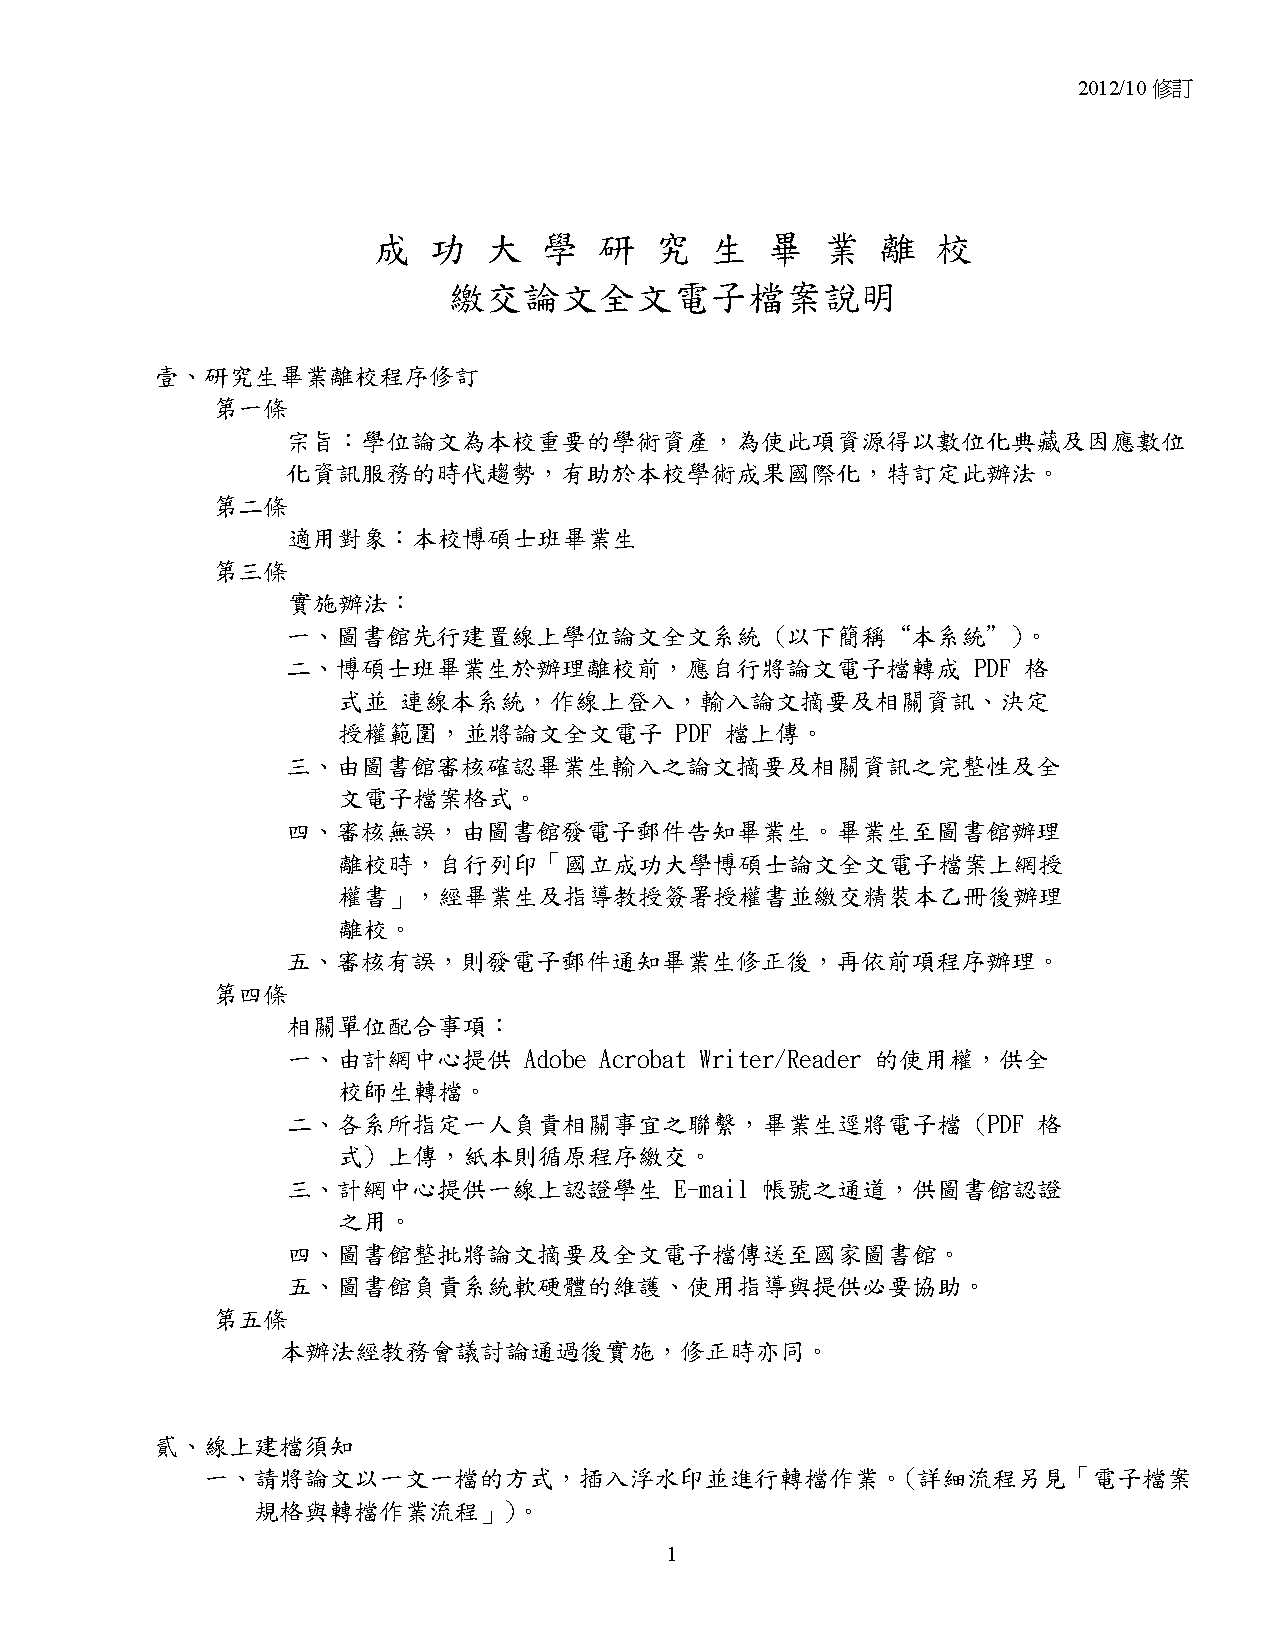
\includepdf[pages=-]{./example/appendix/pdf/2012050004-a.pdf}
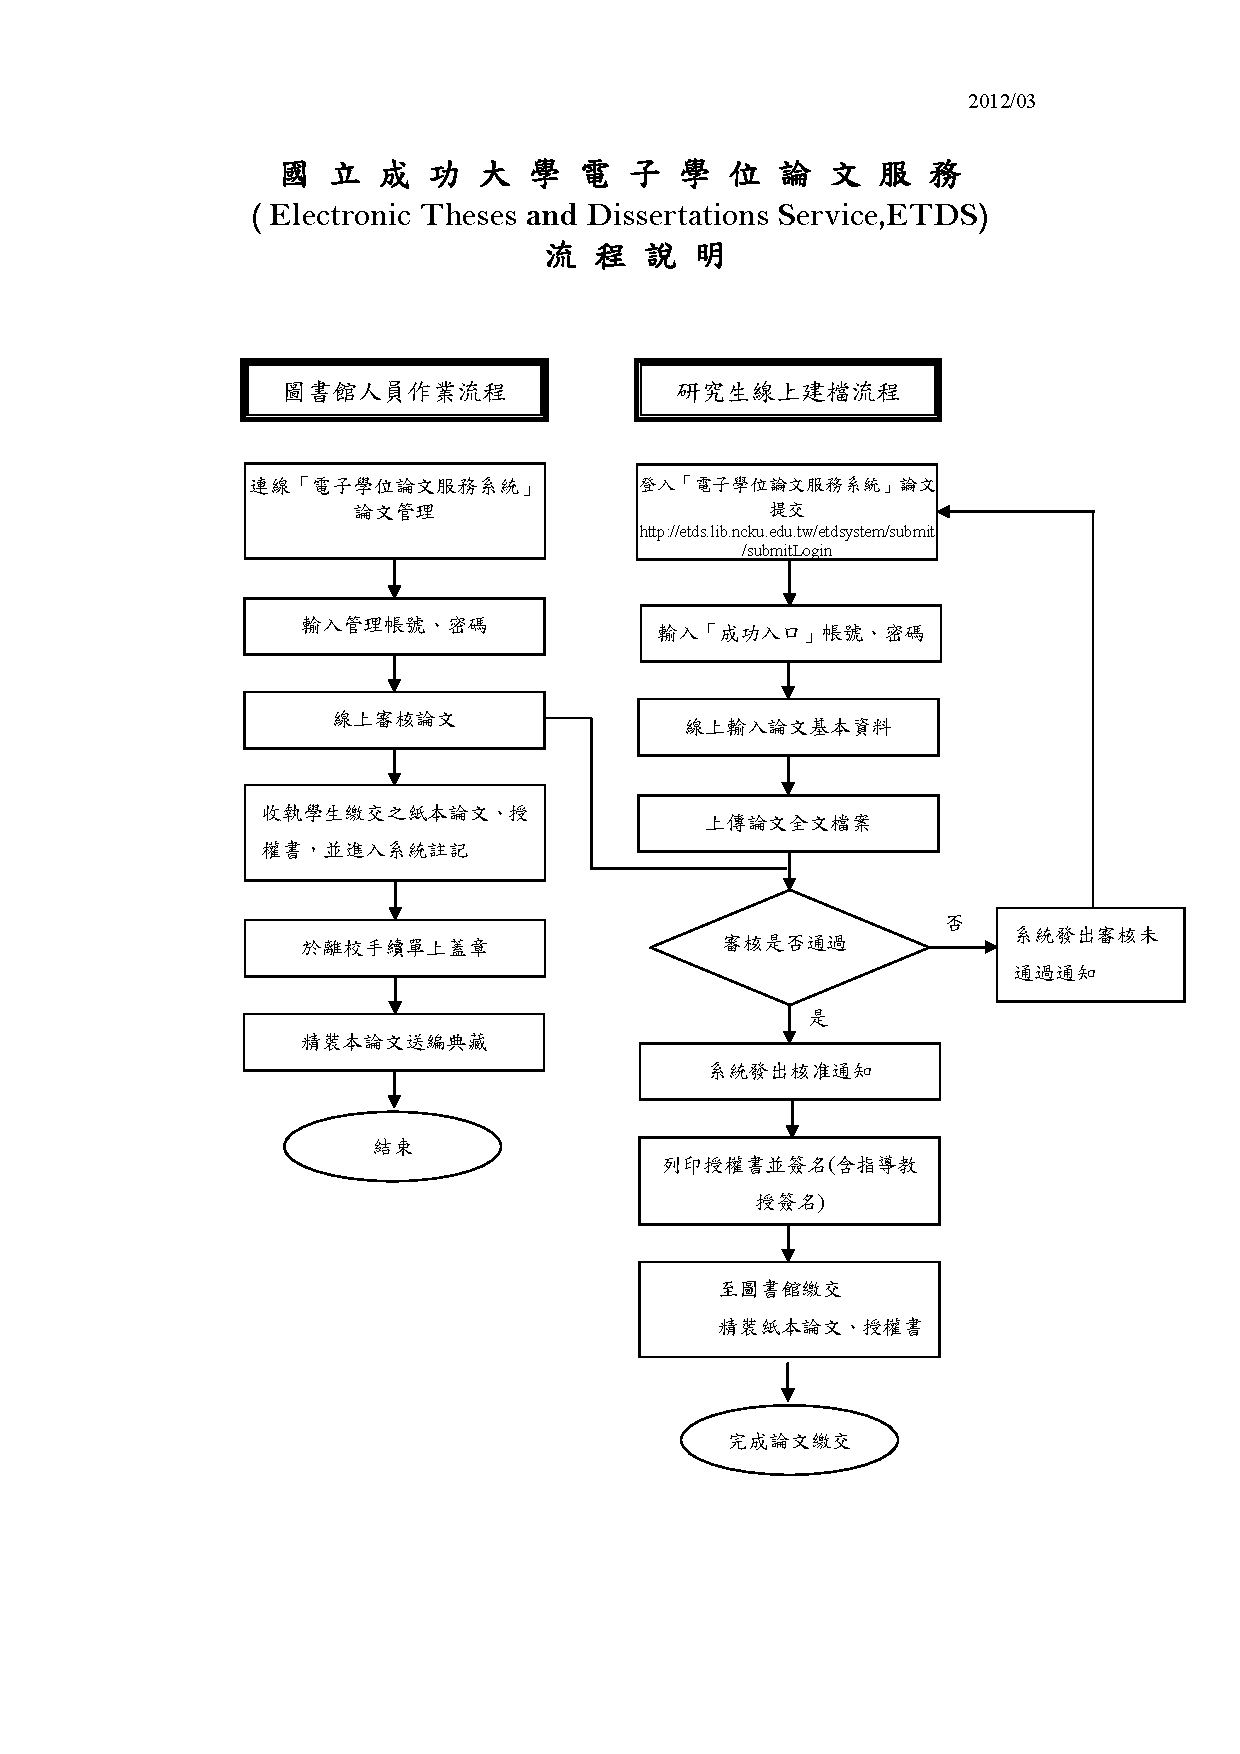
\includepdf[pages=-]{./example/appendix/pdf/2012050006-a.pdf}

% ------------------------------------------------
\EndChapter
% ------------------------------------------------

% ------------------------------------------------
\StartChapter{各系所博碩士撰寫論文須知}{appendix:thesis-spec}
% ------------------------------------------------

這部份資料來源是使用'電子學位論文服務'提供'國立成功大學博碩士學位論文格式規範'\RefBib{web:ncku:thesis-need-to-know}.\\

\setboolean{@twoside}{false}
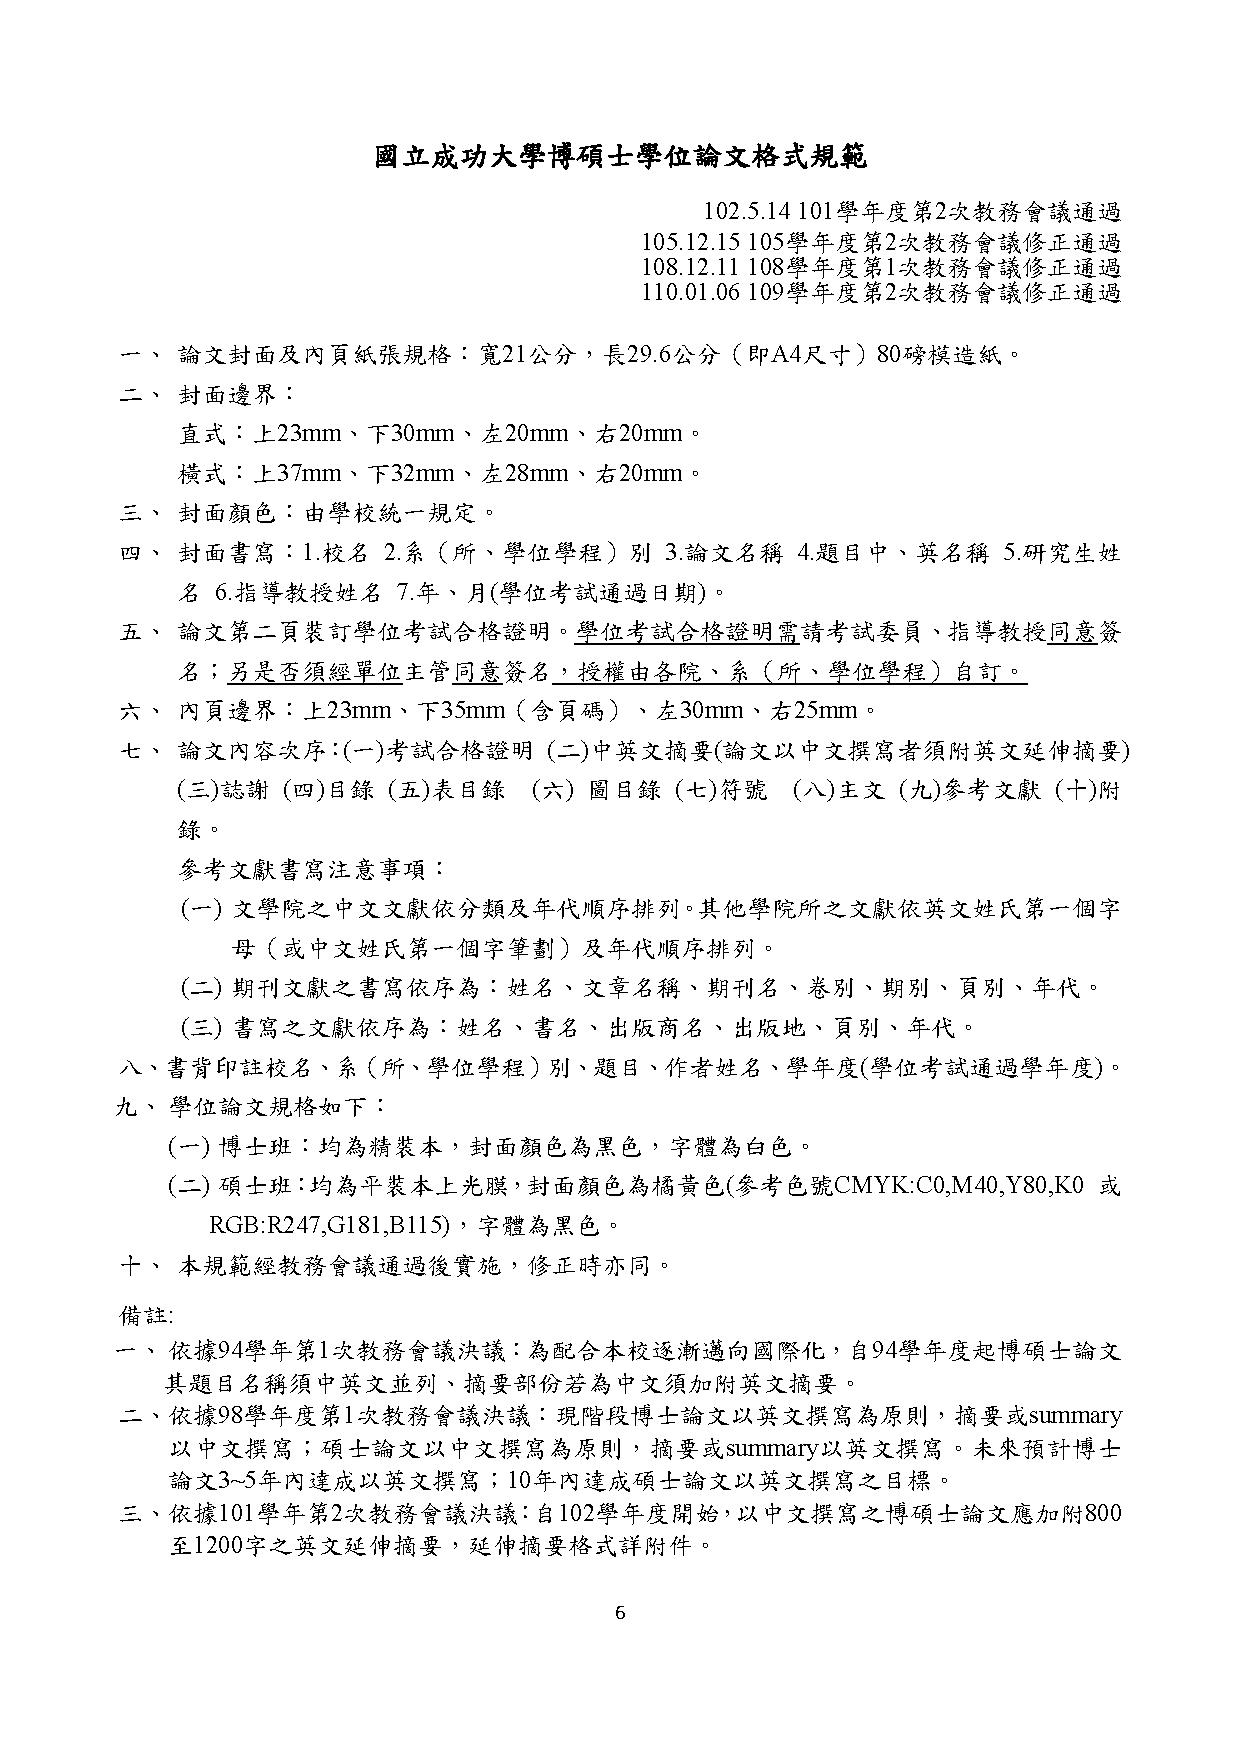
\includepdf[pages=-]{./example/appendix/pdf/thesis-spec-a.pdf}

% ------------------------------------------------
\EndChapter
% ------------------------------------------------

% ------------------------------------------------
\StartChapter{電子論文上傳前檢查事項}{appendix:e-paper_upload}
% ------------------------------------------------

這部份資料來源是使用'電子學位論文服務'中的'電子論文上傳前檢查事項'的'2012090001.pdf'\RefBib{web:lib:upload-things-check}.\\

\setboolean{@twoside}{false}
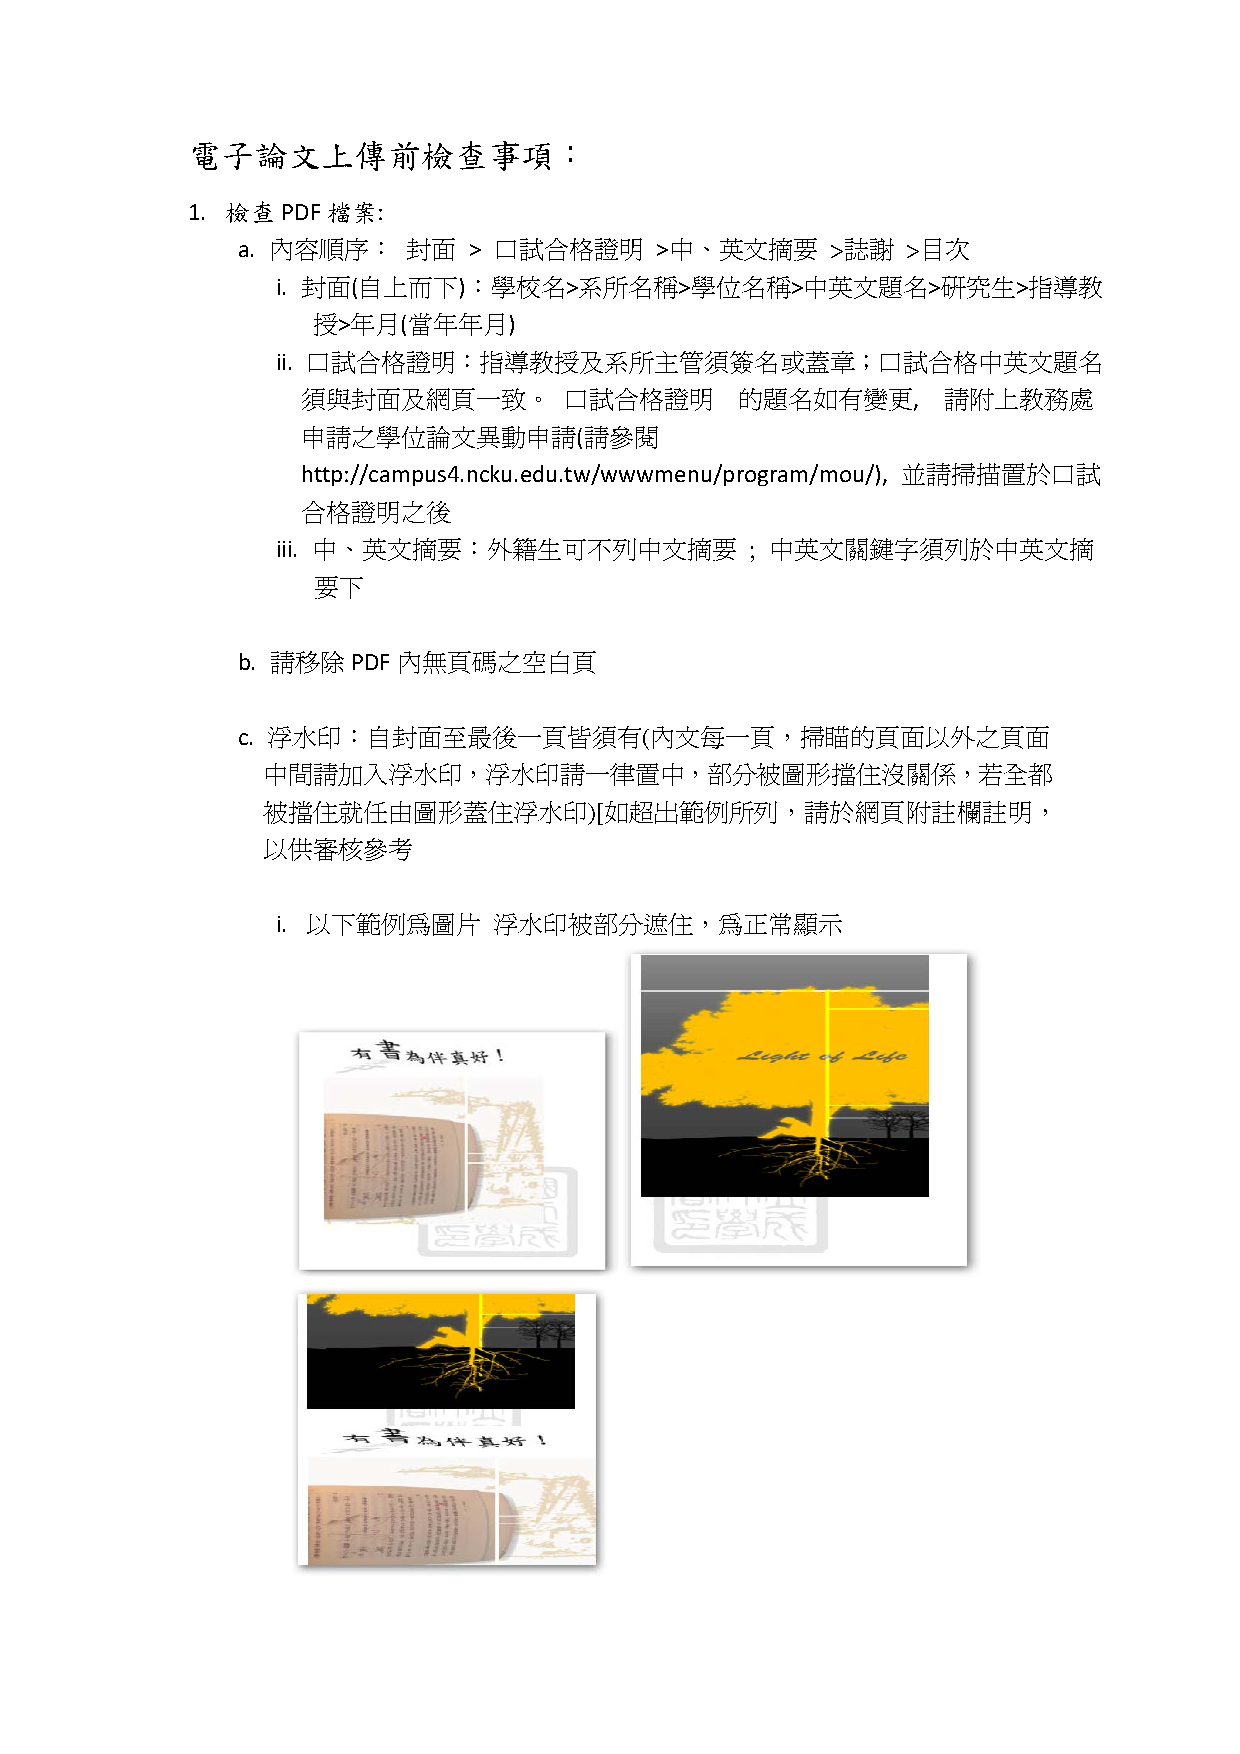
\includepdf[pages=-]{./example/appendix/pdf/2012090001-a.pdf}

% ------------------------------------------------
\EndChapter
% ------------------------------------------------

% ------------------------------------------------
\StartChapter{論文提交說明}{appendix:e-paper_upload_ppt}
% ------------------------------------------------

這部份資料來源是使用'電子學位論文服務'提供的 '2016論文提交說明簡報檔'\RefBib{web:lib:2016-submit-ppt} 修改而成的, 只抽出使用本模版後, 還要做什麼的行為.\\

\setboolean{@twoside}{false}
\includepdf[pages=-]{./example/appendix/pdf/2012050003-short-a}

% ------------------------------------------------
\EndChapter
% ------------------------------------------------

% ------------------------------------------------
\StartChapter{口試注意事項}
% ------------------------------------------------

這部份資料來源是使用本系資訊工程研究所系辦所提供的資料, 雖然內容主要針對本系, 但某些內容都是適合非本系的同學們.

\setboolean{@twoside}{false}
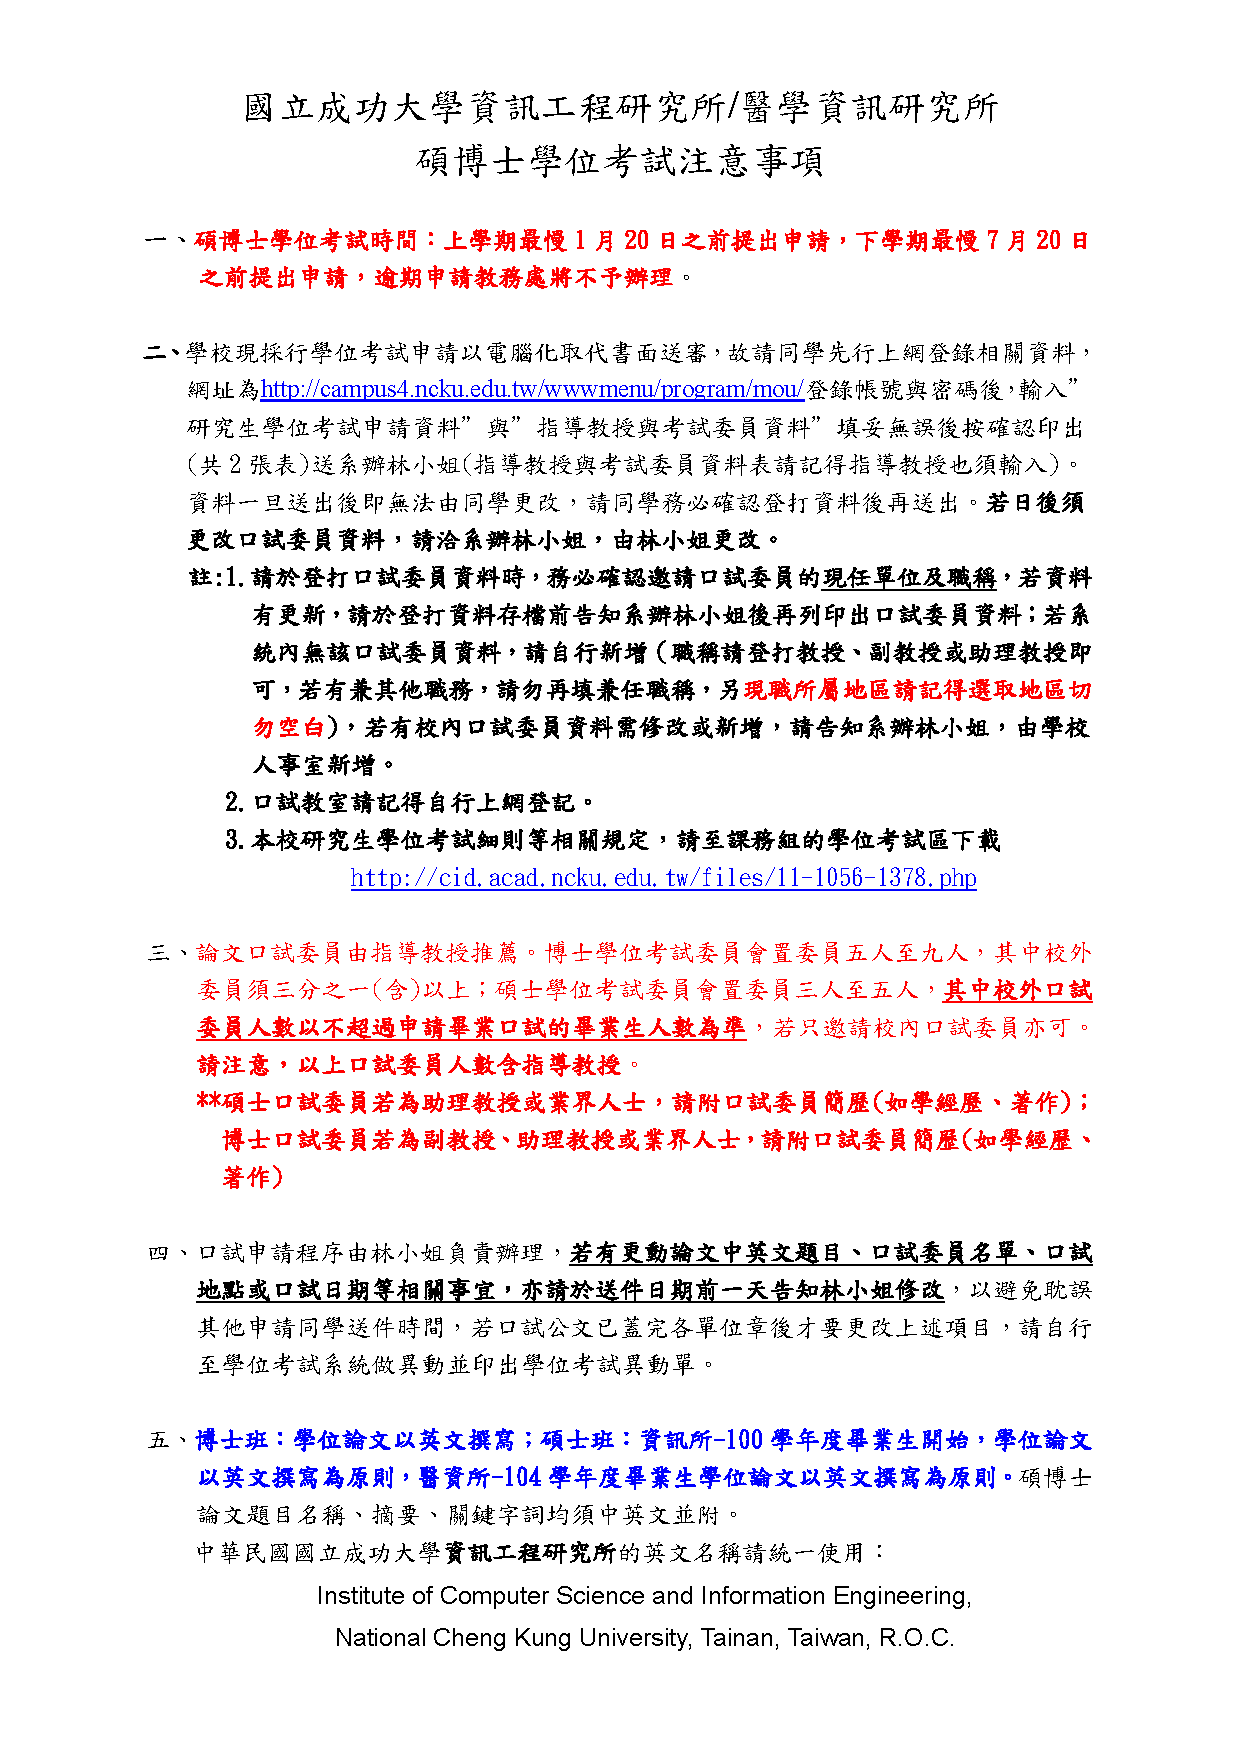
\includepdf[pages=-]{./example/appendix/pdf/oral-1040616-a.pdf}

% ------------------------------------------------
\EndChapter
% ------------------------------------------------

% ------------------------------------------------
\StartChapter{常見問題Q\&A}{appendix:faq}
% ------------------------------------------------

這部份資料來源是使用'電子學位論文服務'提供的'FAQ'\RefBib{web:lib:ETDS-QA}, 用來補充其他Appendix沒提到的一些情報.\\

\setboolean{@twoside}{false}
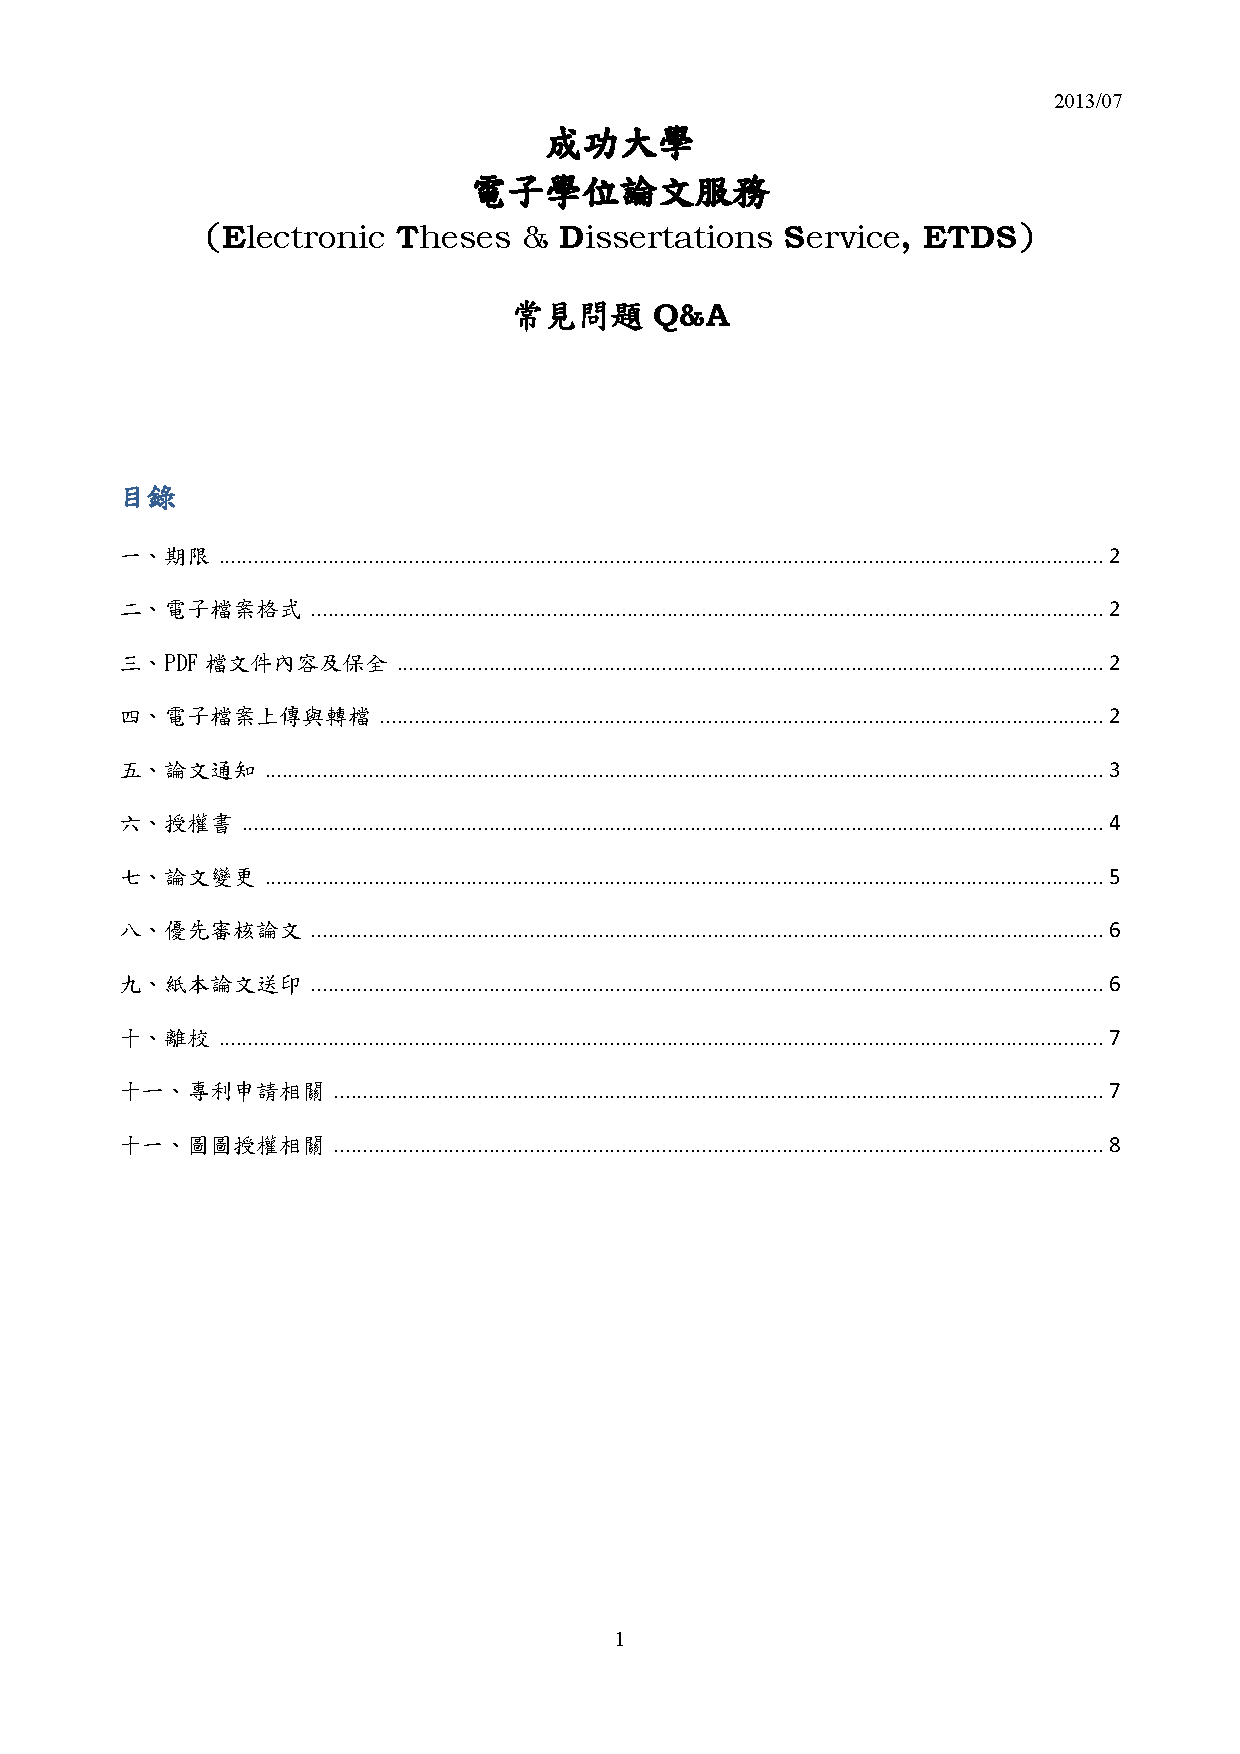
\includepdf[pages=-]{./example/appendix/pdf/2012050009-a.pdf}

% ------------------------------------------------
\EndChapter
% ------------------------------------------------

% ------------------------------------------------
\StartChapter{LaTex Symbol寫法}{appendix:unicode-symbols}
% ------------------------------------------------

這部份資料來源是xeCJK的v3.3.4(2016/02/10)版本中提供的50頁有關所有Symbol的寫法, 極度值得同學們閱讀或在這邊找你所需的Symbols.\\

內容的說明方式為:\\
Symbol: 符號所顯示的樣子\\
USV: 以Unicode方式所代表的這個符號, 例如 `(' 的Unicode寫法為U+0028.\\
Description: 是這符號的名字.\\
Macro(s): 是LaTex使用這符號的寫法.\\

\textbf{P.S: }因為符號數量多, 沒法100\%保證全能使用.

\setboolean{@twoside}{false}
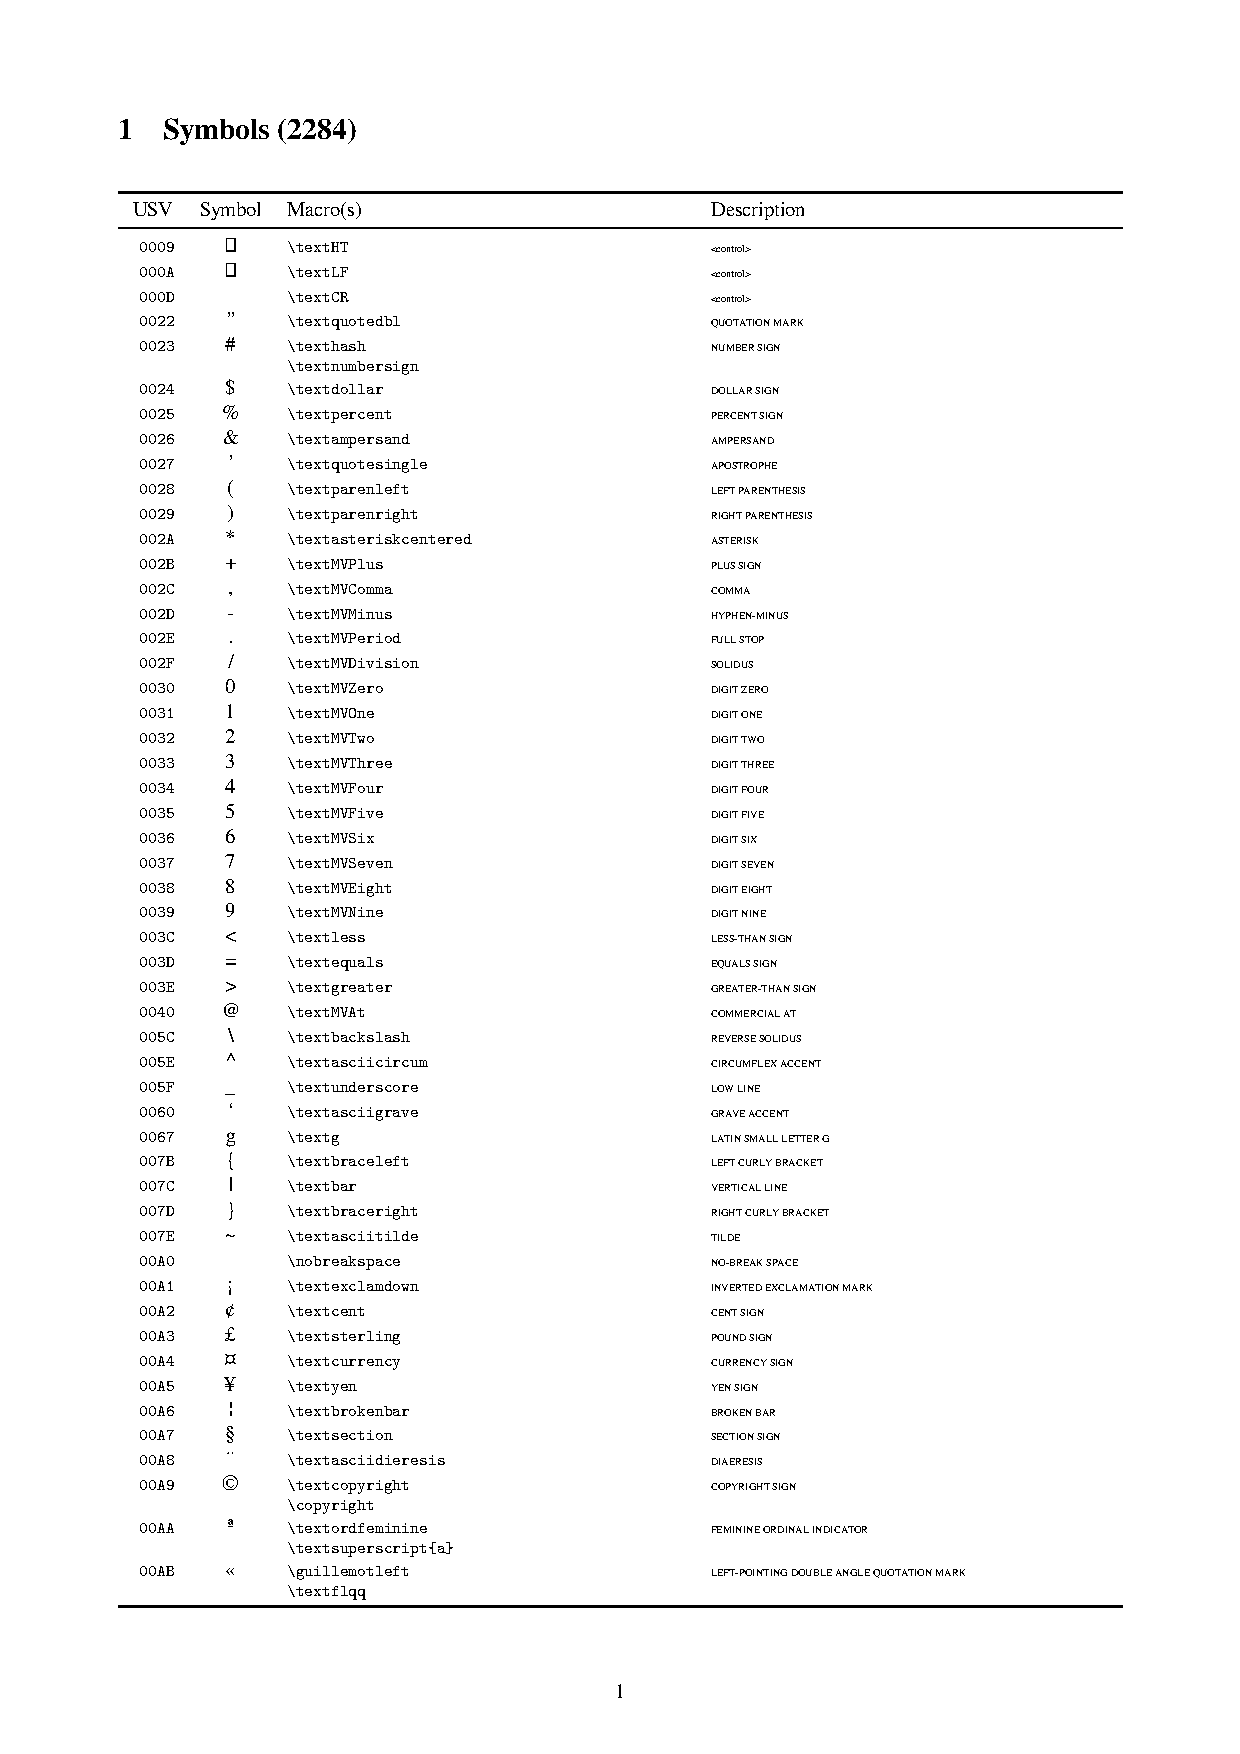
\includepdf[pages=-]{./example/appendix/pdf/xunicode-symbols.pdf}

% ------------------------------------------------
\EndChapter
% ------------------------------------------------


% ------------------------------------------------
\EndAppendix
% ------------------------------------------------


% ------------------------------------------------
